% Copyright (C) 2004-2006 Jed Brown and Ed Bueler
%
% This file is part of Pism.
%
% Pism is free software; you can redistribute it and/or modify it under the
% terms of the GNU General Public License as published by the Free Software
% Foundation; either version 2 of the License, or (at your option) any later
% version.
%
% Pism is distributed in the hope that it will be useful, but WITHOUT ANY
% WARRANTY; without even the implied warranty of MERCHANTABILITY or FITNESS
% FOR A PARTICULAR PURPOSE.  See the GNU General Public License for more
% details.
%
% You should have received a copy of the GNU General Public License
% along with Pism; if not, write to the Free Software
% Foundation, Inc., 51 Franklin St, Fifth Floor, Boston, MA  02110-1301  USA

\documentclass[11pt,final]{amsart}

\newcommand{\PISMREV}{141}
\newcommand{\PETSCREV}{2.3.3-p2}

\addtolength\topmargin{-.1in}
\addtolength\textheight{0.3in}
\addtolength{\oddsidemargin}{-.65in}
\addtolength{\evensidemargin}{-.65in}
\addtolength{\textwidth}{1.3in}
\newcommand{\normalspacing}{\renewcommand{\baselinestretch}{1.1}\tiny\normalsize}
\newcommand{\tablespacing}{\renewcommand{\baselinestretch}{1.0}\tiny\normalsize}
\normalspacing

\usepackage{bm,url,xspace,verbatim}
\usepackage{amssymb,amsmath}
\usepackage[final,pdftex]{graphicx}
\usepackage[pdftex]{hyperref}

\renewcommand{\t}[1]{\texttt{#1}}
\newcommand{\Matlab}{\textsc{Matlab}\xspace}
\newcommand{\bU}{\mathbf{U}}
\newcommand{\eps}{\epsilon}

% note \beginV and \Vend are a pair, but they must be used as follows:
%   \beginV
%      ... stuff
%   \end{verbatim}
%   \Vend
% that is, "\end{verbatim}" still has to appear on a line by itself with no leading spaces
%\newcommand{\Vend}{ \rule{4.6in}{0.1mm}\end{quote} }
%\newcommand{\beginV}{ \begin{quote}\rule{4.6in}{0.1mm}\begin{verbatim} }
\newcommand{\Vend}{ \rule{4.6in}{0.1mm}\end{quote}\normalsize }
%\newcommand{\beginV}{ \small\begin{quote}\rule{4.6in}{0.1mm}\begin{verbatim} }
\newcommand{\beginV}{ \scriptsize\begin{quote}\rule{4.6in}{0.1mm}\begin{verbatim} }

\newcommand{\Vfile}[1]{ \begin{quote}\rule{4.6in}{0.1mm} \verbatiminput{#1} \rule{4.6in}{0.1mm}\end{quote} }

%\makeindex

\title[PISM User's Manual]{PISM, a \underline{P}arallel \underline{I}ce \underline{S}heet \underline{M}odel: \\ User's Manual and Reference}

\author[]{Ed $\text{Bueler}^\ast$, Jed Brown, and Nathan Shemonski}

\date{\today.  $\phantom{|}^\ast$\texttt{ffelb\@@uaf.edu}.  Based on PISM revision \PISMREV\,and PETSC release \PETSCREV.  \\\tiny Get PISM by Subversion: \texttt{svn co http://svn.gna.org/svn/pism/trunk pism}; update to latest version by \texttt{svn update}.} 

\begin{document}
\maketitle
\thispagestyle{empty}
%\tablespacing

\vspace{2.0in}
\begin{center}
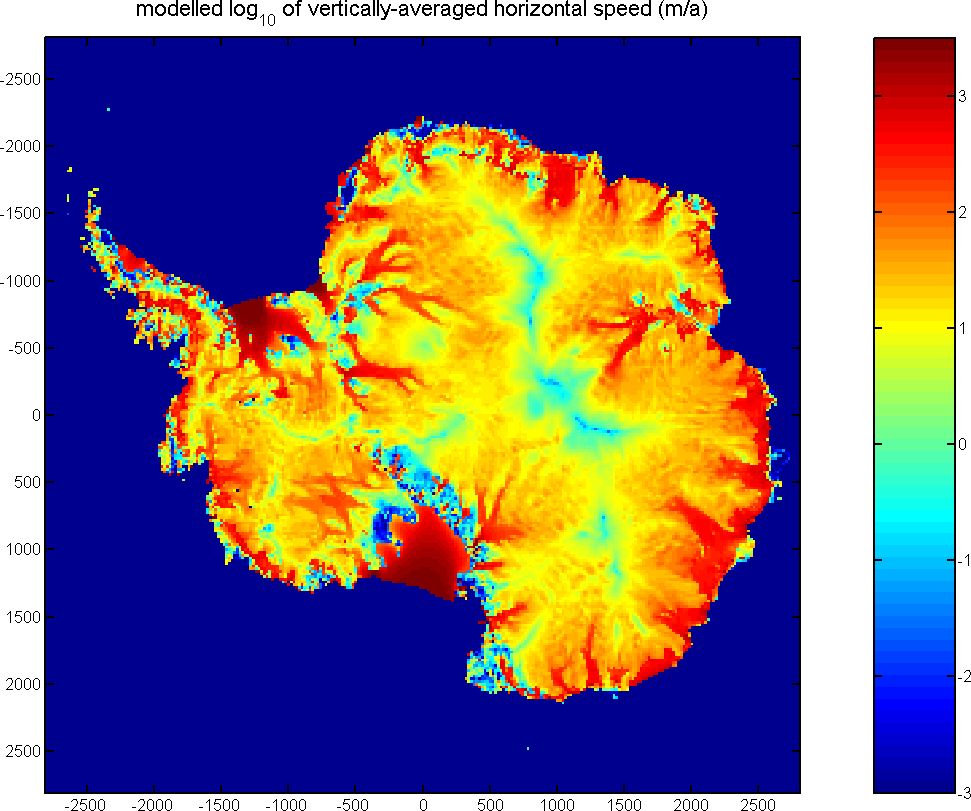
\includegraphics[height=2.7in,keepaspectratio=true]{figs/ant153k_mv100_speed}
\end{center}

\newpage
\phantom{bob}
\vspace{2in}
\begin{quote}
\textsl{Copyright (C) 2004--2007 Jed Brown and Ed Bueler and Nathan Shemonski}
\medskip

\noindent \textsl{This file is part of PISM.}
\medskip

\noindent \textsl{PISM is free software; you can redistribute it and/or modify it under the terms of the GNU General Public License as published by the Free Software Foundation; either version 2 of the License, or (at your option) any later version.}
\medskip

\noindent \textsl{PISM is distributed in the hope that it will be useful, but WITHOUT ANY WARRANTY; without even the implied warranty of MERCHANTABILITY or FITNESS FOR A PARTICULAR PURPOSE.  See the GNU General Public License for more details.}
\medskip

\noindent \textsl{You should have received a copy of the GNU General Public License along with PISM; see \emph{\texttt{pism/COPYING}}; if not, write to the Free Software Foundation, Inc., 51 Franklin St, Fifth Floor, Boston, MA  02110-1301 USA}
\end{quote}
\vspace{1in}
\normalspacing

\centerline{\textsc{Acknowledgements}}
\bigskip

The NASA Cryospheric Sciences Program supported this research with grant NAG5-11371.  Dave Covey and Don Bahls have been the best possible system administrators for the machines on which we have developed PISM.  Thanks to Art Mahoney for helpful comments on the manual and the installation process.

We also want to thank PISM users whose questions and comments have contributed to improving PISM and this manual.

\newpage
\setcounter{tocdepth}{2}
\tableofcontents


\newpage
\section{Installation}\label{sect:install}

\renewcommand{\labelenumi}{\textbf{\arabic{enumi}.}~}
\begin{enumerate}
\item You will need a UNIX system with internet access.  A GNU/Linux environment will be easiest but other UNIX versions have been used successfully.  Package management systems are useful for installing many of the tools below, \emph{but} neither PISM itself nor up-to-date PETSc distributions are currently available in the Debian repositories.  You will need Python (\url{http://www.python.org/}) and Subversion (\url{http://subversion.tigris.org/}) installed, but these are included in all current Linux distributions.

\item To use the graphical output of PISM, which we recommend, you will need an X Windows server \emph{and} the developers' version of X11, which will contain the needed header files.  The relevant development package in Debian is called \verb|xorg-dev|.

\item PISM uses NetCDF (= \emph{network Common Data Form}; \url{http://www.unidata.ucar.edu/software/netcdf/}) for an input and output file format.   Install it using the instructions at the NetCDF webpage or using a package management system.  You will need the development version (package) which includes the header files; this is the \verb|netcdfg-dev| package in the Debian repositories.

\item PISM uses the GSL (= \emph{GNU Scientific Library}; \url{http://www.gnu.org/software/gsl/}) for certain numerical calculations and special functions.  Install it using the instructions at the GSL webpage or using a package management system.  You will need the development version (package) which includes header files; this is the \verb|libgsl0-dev| package in the Debian repositories.

\item PISM optionally uses the ``FFTW'' library (FFTW = \emph{Fastest Fourier Transform in the West}; \url{http://www.fftw.org/}) in approximating the deformation of the solid earth under ice loads \cite{BLKfastearth}.  If you want the functionality of this earth model, which is coupled to the ice flow and which we recommend, install FFTW or check that it is installed already.   In particular, get the development version with header files, which is \verb|fftw3-dev| in Debian.   If FFTW is \emph{not installed}, however, turn off PISM's attempt to build with it by setting the environment variable \verb|WITH_FFTW=0|.   If this library is absent, all of PISM will work \emph{except} for the bed deformation model described in the paper \cite{BLKfastearth}.

\item You will need a version of MPI (= \emph{Message Passing Interface}; \url{http://www-unix.mcs.anl.gov/mpi/}).  Your system may have an existing MPI installation in which case the path to the MPI directory will be used when installing PETSc below.  Otherwise we recommend that you allow PETSc to download MPICH2 (\url{http://www-unix.mcs.anl.gov/mpi/mpich2/}) as part of the PETSc configure process (next).  In either case, once MPI is installed, you will want to add the MPI \verb|bin| directory to your path so that you can invoke MPI using the \verb|mpiexec| or \verb|mpirun| command.  For example, you can add it with the statement

\verb|export PATH=/home/user/mympi/bin:$PATH|  \qquad (for \verb|bash| shell)

\noindent or

\verb|setenv PATH /home/user/mympi/bin:$PATH|  \qquad (for \verb|csh| or \verb|tcsh| shell).

\noindent Such a statement can, of course, appear in your \verb|.bashrc|, \verb|.profile|, or \verb|.cshrc| file so that there is no need to retype it each time you use MPI.

\medskip
\centerline{\emph{From now on this manual will assume use of} bash.}
\medskip

\item PISM uses PETSc (= \emph{Portable Extensible Toolkit for Scientific computation}; \url{http://www-unix.mcs.anl.gov/petsc/petsc-2/index.html}).  As mentions of this library will occur frequently in this manual, note ``PETSc'' is pronounced ``pet-see''.  Download the PETSc source by grabbing the current gzipped tarball at \url{http://www-unix.mcs.anl.gov/petsc/petsc-as/download/index.html}.  PISM requires a version of PETSc which is \texttt{\PETSCREV} or later.   The ``lite'' form of PETSc is fine if you are willing to depend on an internet connection for accessing the PETSc documentation. 

You should configure and build PETSc \emph{essentially} as described on the installation page \url{http://www-unix.mcs.anl.gov/petsc/petsc-2/documentation/installation.html}, but it might be best to read the following comments on the PETSc configure and build process first:

\renewcommand{\labelenumii}{(\roman{enumii})}\begin{enumerate}
\item Untar in your preferred location, but note PETSc should \emph{not} be configured (next) using root privileges.  Note that you will need to define the environment variable \verb|PETSC_DIR| before configuring PETSc (next).  For instance, once you have entered the PETSc directory just untarred, \verb|export PETSC_DIR=|$\phantom{!}^\backprime \mathtt{pwd}^\backprime$.  (Note the use of the backprime (\emph{accent-grave}) character, and not the single apostrophe \verb|'|.)

\item When you run the configure script in the PETSc directory, the following options are recommended; note PISM uses shared libraries by default:

\verb|$  ./config/configure.py --with-shared --with-c-support --with-clanguage=cxx|

Note that there is no PISM use of Fortran, and that it is sometimes convenient to have PETSc grab a local copy of BLAS and LAPACK rather than using the system-wide version.  So one may add ``\verb|--with-fortran=0| \verb|--download-c-blas-lapack=1|'' to the other configure options.

\item If there is an existing MPI installation, for example at \verb|/home/user/mympi/|, one can point PETSc to it by adding the option \verb|--with-mpi-dir=/home/user/mympi/|.  The path used in this option must have MPI executables \verb|mpicxx| and \verb|mpicc|, and either \verb|mpiexec| or \verb|mpirun|, in subdirectory \verb|bin/| and MPI library files in subdirectory \verb|lib/|.

\item On the other hand, it seems common that one needs to tell PETSc to download MPI into a place it understands, even if there is an existing MPI.  If you get messages suggesting that PETSc cannot configure using your existing MPI, you might try \verb|configure.py| with option \verb|--download-mpich=1|.

\item Configuration of PETSc for a batch system requires special procedures described at the PETSc documentation site.  One starts with a configure option \verb|--with-batch=1|.  See the ``Installing on machine requiring cross compiler or a job scheduler'' section of the installation page \url{http://www-unix.mcs.anl.gov/petsc/petsc-as/documentation/installation.html}.

\item  Configuring PETSc takes many minutes even when everything goes smoothly.   A value for the environment variable \verb|PETSC_ARCH| will be reported at the end of the configure process; take note of this value.  (Note that a previously installed PETSc can be reconfigured with a new \verb|PETSC_ARCH| if necessary.)

\item  After \verb|configure.py| finishes, you will need to \verb|make all test| in the PETSc directory and watch the result.  If the X Windows system is functional some example viewers will appear; as noted you will need the X header files for this to work.

\item Finally, you will want to set the \verb|PETSC_DIR| and the \verb|PETSC_ARCH| environment variables in your \verb|.profile| or \verb|.bashrc| file.  Also remember to add the MPI \verb|bin| directory to your \verb|PATH|.  For instance, if you used the option \verb|--download-mpich=1| in the PETSc configure, the MPI \verb|bin| directory will have a path like \verb|$PETSC_DIR/| \verb|externalpackages/mpich2-1.0.4p1/$PETSC_ARCH/bin/|.  Therefore the lines 

\small
\verb|export PETSC_DIR=/home/user/petsc-2.3.3-p2/|

\verb|export PETSC_ARCH=linux-gnu-c-debug|

\verb|export PATH=$PETSC_DIR/externalpackages/mpich2-1.0.4p1/$PETSC_ARCH/bin/:$PATH|
\normalsize

\noindent could appear in one of those files.
\end{enumerate}
\end{enumerate}

\bigskip
See Table \ref{tab:PISMdepends} for a summary of the dependencies on external libraries, including those mentioned so far.

\medskip
At this point you have configured the environment which PISM needs.  You are ready to build PISM itself, which is much quicker procedure!
\bigskip

\begin{enumerate}\setcounter{enumi}{5}
\item \label{getPISMstep} Get the latest source for PISM by

\verb|$  svn co http://svn.gna.org/svn/pism/trunk pism|

\noindent A directory called ``\verb|pism/|'' will be created.  Note that in the future when you enter that directory, \verb|svn update| will update to the latest revision of PISM.

\item Build PISM:

\verb|cd pism|

\verb|make|

\verb|make install|

\noindent  Note that the ``\verb|install|'' is local to the \verb|pism| directory and does not require root permission.  Several executables, including \verb|pismv|, \verb|pisms|, and \verb|pismr|, should appear in the \verb|pism/bin/| subdirectory.  (Please report any problems you meet at this stage by sending us the output: \verb|ffelb@uaf.edu|.)  

\item PISM executables can be run most easily by adding the directories \verb|pism/bin/| and \verb|pism/test/| to your \verb|PATH|.  The former directory contains the major PISM executables while the latter contains several useful scripts.  For instance, this command can be done in the \verb|bash| shell or in your \verb|.bashrc| file:

\verb|export PATH=/home/user/pism/bin/:/home/user/pism/test/:$PATH|
\end{enumerate}

\bigskip
You are done with installation at this point.  The next few items are recommended as they allow you to observe that PISM is functioning correctly.
\bigskip

\begin{enumerate}\setcounter{enumi}{9}
\item \label{serialpismvrun} Try a serial verification run of PISM:

\verb|$  pismv -test G -y 100|

\noindent If you see some output and a final 

\verb|Writing model state to file 'verify.nc' ... done|

\noindent then PISM completed successfully.  Note that at the end of this run you will get measurements of the difference between the numerical result and the exact solution \cite{BBL}.

\item Try the MPI four processor version of the above run:

\verb|$  mpiexec -n 4 pismv -test G -y 100|

\noindent This should work even if there is only one actual processor on your machine, in which case MPI will run multiple processes on the one processor, naturally.  The reported errors should be very nearly the same as the serial run above, but the results should appear faster (if there really are four processors)!

\item Try a verification run on a finer vertical grid while watching the diagnostic views which use Xwindows:

\verb|$  pismv -test G -Mz 201 -y 2000 -d HTc|

\noindent When using such diagnostic views and \verb|mpiexec| the additional final option \verb|-display :0| is sometimes required to enable MPI to use Xwindows:

\verb|$  mpiexec -n 2 pismv -test G -Mz 201 -y 2000 -d HTc -display :0|

\item Run a verification test of the ice stream code:

\verb|$  pismv -test I -Mx 5 -My 401 -verbose|

\noindent This runs a rather different part of the PISM code and then compares the numerical result to the exact solution appearing in \cite{SchoofStream}.

\item Run a Python script for a basic suite of verifications:

\verb|$  verifynow.py|

\noindent If you would like us to confirm that PISM is working as expected please save the one page or so of output from this script and send it to us (\verb|ffelb@uaf.edu|).  See section \ref{sect:verif} for more on PISM verification.
\end{enumerate}
\bigskip

Have fun!

At this stage you can do the EISMINT II tests and some verification tests without further downloads.  Sections \ref{sect:valid} and \ref{sect:real} describe using PISM to model real ice sheets (and shelves) based on freely available data already on the web.  

Naturally, setting up PISM to model real ice sheets will generally require techniques not be covered in this manual.  It may require the writing of additional source code, which for PISM means writing a derived class of the base \verb|IceModel| class defined by the PISM C++ source code.  Use of PISM for real ice sheet modelling is something we welcome questions about and will attempt to help with.

A final reminder with respect to installation:  Once you have checked out a copy of PISM using Subversion, as in step \ref{getPISMstep} above, you can update it to the latest version by \verb|svn update| in the \verb|pism/| directory, after which you will want to \verb|make| again, of course.

\begin{table}[h]
\caption{Dependencies for PISM, listed alphabetically.  Note developers' versions, which include the relevant header files, are needed for FFTW, GSL, and NetCDF.}\label{tab:PISMdepends}
\small
\begin{tabular}{@{}llll}\hline
\textbf{Library} & \textbf{Site} & \textbf{Required?} & \textbf{Comment} \\
\textbf{/Program} &  &  &  \\ \hline
FFTW & \url{www.fftw.org} & \emph{recommended} & if not present  \\
 & & & \quad set \verb|WITH_FFTW=0| \\
GSL & \url{www.gnu.org/software/gsl} & \emph{required} &  \\
\LaTeX & \url{http://www.latex-project.org/} & \emph{optional} & only used for rebuilding \\
& & & manual from source \\
Matlab & \url{www.mathworks.com} & \emph{optional} & only used for alternate\\
& & & display of results \\
MPI & \url{www-unix.mcs.anl.gov/mpi} & \emph{required} & \\
NetCDF & \url{www.unidata.ucar.edu/software/netcdf} & \emph{required} & \\
PETSc & \scriptsize \url{www-unix.mcs.anl.gov/petsc/petsc-2/index.html} \small & \emph{required} & version $\ge$ 2.3.3-p2 \\
Python & \url{python.org} & \emph{required} & \\
Subversion & \url{subversion.tigris.org} & \emph{required} & \\
\hline
\normalsize
\end{tabular}
\end{table}


\clearpage\newpage
\section{Getting started}\label{sect:start}

\subsection{Running the EISMINT II tests}  PISM's purpose is the realistic simulation of ice sheets.  But real ice sheet simulations require real data.  And real data is something we cannot generally distribute under the GNU Public License.  (Real ice sheet and ice shelf data \emph{is} available on the web as part of the EISMINT intercomparison efforts; see sections \ref{sect:valid} and \ref{sect:real}.)  So this section describes how PISM does experiment F in the EISMINT II thermomechanical coupling intercomparison \cite{EISMINT00}.  In this experiment one tries to approximate an unstable equilibrium of the thermomechanically coupled differential equations for a shallow, grounded ice sheet.  One gets the infamous ``spokes'' \cite{BBL,PayneBaldwin}.  The prescribed grid has 60 subintervals in each direction, with each subinterval of length 25km, but the vertical grid is not prescribed.  Runs are for 200,000 model years.

PISM always allows choice of the grid in three dimensions.  A runtime option chooses the number of grid points in each direction; the number of points is one greater than the number of subintervals.  We choose the standard 25km grid in the horizontal and use 201 grid points in the vertical for a 25 m (equally-spaced) grid because the computational box is 5000 m for EISMINT II experiment F in PISM.  The executable is ``\t{pisms}'', a name which has trailing ``\t{s}'' for the ``simplifed geometry mode'' of PISM.  Here is a short 2000 year run.

\small\begin{quote}\begin{verbatim}
$  pisms -eisII F -Mx 61 -My 61 -Mz 201 -y 2000
PISMS (simplified geometry mode)
initializing EISMINT II experiment F ...
  [computational box for ice: ( 1500.00 km) x ( 1500.00 km) x ( 5000.00 m)]
  [grid cell dimensions     : (   25.00 km) x (   25.00 km) x (   25.00 m)]
running EISMINT II experiment F ...
$$$$$      YEAR (+    STEP[N$]):     VOL    AREA    MELTF     THICK0     TEMP0
$$$$$      0.00 (+  0.0000[0 ]):   0.000   0.000    0.000      0.000   223.150
$v$tf     60.00 (+ 60.0000[0m]):   0.017   0.628    0.000     30.000   223.150
$v$tf    120.00 (+ 60.0000[0m]):   0.034   0.628    0.000     60.000   223.538
$v$tf    180.00 (+ 60.0000[0m]):   0.051   0.628    0.000     90.000   223.869
$v$tf    240.00 (+ 60.0000[0m]):   0.068   0.628    0.000    120.000   224.162
$v$tf    300.00 (+ 60.0000[0m]):   0.085   0.631    0.000    150.000   224.425
$v$tf    360.00 (+ 60.0000[0m]):   0.102   0.631    0.000    180.000   224.667
...
$v$tf   1920.00 (+ 60.0000[0m]):   0.545   0.631    0.000    960.000   228.389
$v$tf   1980.00 (+ 60.0000[0m]):   0.562   0.631    0.000    990.000   228.487
$v$tf   2000.00 (+ 20.0000[0e]):   0.568   0.631    0.000   1000.000   228.520
done with run ... Writing model state to file `simp_exper.nc' ... done.
\end{verbatim}
\end{quote}\normalsize

This should have taken less than 30 seconds on any modern computer.  In a moment we will address the standard output information provided by PISM, shown above.  For now we simply illustrate how to restart and complete the 200,000 year run.  Note that the model state was stored in a file with a default name ``\texttt{simp\underline{ }exper.nc}''.  We will see in a moment an example which uses an option to name the output file, and an option to choose its format.  The above was a single processor run, but let's suppose we have a four processor machine; the following should work as stated on a single processor machine under most MPI installations.  Let's run things in the background so we can continue to experiment.

\small\begin{quote}\begin{verbatim}
$  mpiexec -n 4 pisms -eisII F -if simp_exper.nc -y 198000 \
  -o eisIIF200k >> eisIIF.out &
\end{verbatim}
\end{quote}\normalsize

\noindent We have named the output.  The file \verb|eisIIF200k.nc| (NetCDF format) will appear at the end of this run, which will take at least an hour on a four processor computer.  One can, however, view the redirected standard output by \verb|less eisIIF.out| as the job is running in the background.  Also ``\t{top}'' is a convenient tool to see processor usage during the run.  (If one kills the run with \verb|pkill pism|, which sends a \verb|SIGTERM| signal to all \verb|pism| processes, then the run will stop with the model state saved in the named output file \verb|eisIIF200k.nc| even though it will not represent the state at 200,000 years.)

While the above is running in the background, let's actually view the model state during a few time steps by starting from the saved 2000 year state.  We use PISM's ``diagnostic viewers'', which are PETSc viewers working under Xwindows:

\small\begin{quote}\begin{verbatim}
$  pisms -eisII F -if simp_exper.nc -y 200 -d HTt
PISMS (simplified geometry mode)
initializing from NetCDF format file  simp_exper.nc  ...
  [computational box for ice: ( 1500.00 km) x ( 1500.00 km) x ( 5000.00 m)]
  [grid cell dimensions     : (   25.00 km) x (   25.00 km) x (   25.00 m)]
running EISMINT II experiment F ...
$$$$$       YEAR (+     STEP[N$]):     VOL    AREA    MELTF     THICK0     TEMP0
$$$$$   2000.000 (+  0.00000[0 ]):   0.568   0.631    0.000   1000.000   228.520
$v$tf   2060.000 (+ 60.00000[0m]):   0.585   0.631    0.000   1030.000   228.616
$v$tf   2120.000 (+ 60.00000[0m]):   0.602   0.631    0.000   1060.000   228.710
$v$tf   2180.000 (+ 60.00000[0m]):   0.619   0.631    0.000   1090.000   228.804
$v$tf   2200.000 (+ 20.00000[0e]):   0.625   0.631    0.000   1100.000   228.834
done with run ... Writing model state to file `simp_exper.nc' ... done.
\end{verbatim}
\end{quote}\normalsize

Three figures should appear and be refreshed at each time step.  One figure is a map-plane view of thickness, another is a map-plane view of the basal temperature in Kelvin, and third there is a graph of height above the bed versus temperature.  When the above 200,000 year run above finishes, on can display the result by \verb|pisms -eisII F| \verb|-if eisIIF200k.nc -y 200 -d HTt|.  In that case the result shown in figure \ref{fig:screenshot} will appear.
\medskip

\begin{figure}[ht]
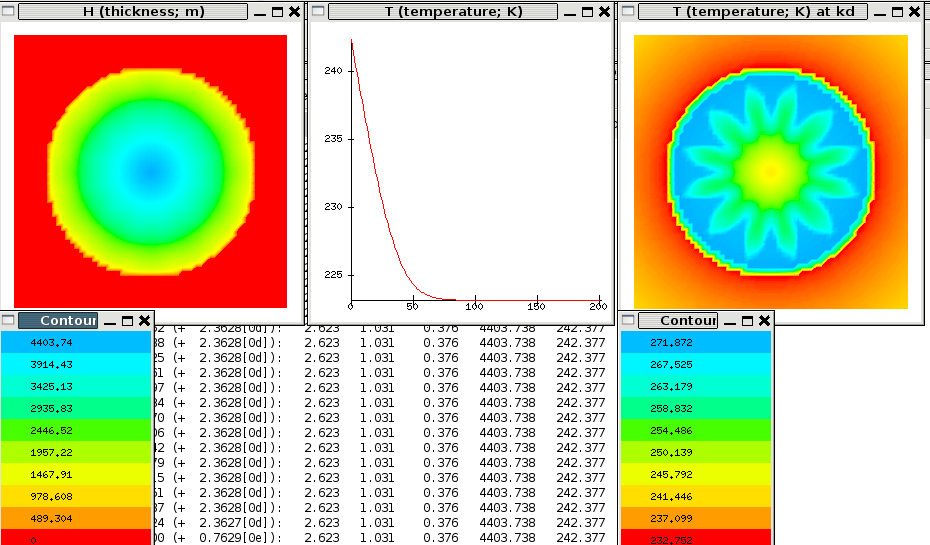
\includegraphics[height=3.2in,keepaspectratio=true]{figs/eisIIFshot}
\caption{Diagnostic figures at the end of a 200,000 year EISMINT II experiment F run, showing the famous spokes.}
\label{fig:screenshot}
\end{figure}

At each time step PISM shows a summary of the model state using a few numbers.  The format of the summary is

\small\verb|$$$$$      YEAR (+    STEP[N$]):     VOL    AREA    MELTF     THICK0     TEMP0|\normalsize

\noindent The first five columns are flags telling the user which quantities are being updated at each time step.  A dollar sign appears if the quantity does not update.  From the left the positions are: [\t{b\$}] for bed elevation, [\t{vV\$}] for velocity, [\t{g\$}] for grain size, [\t{t\$}] for temperature and age (which are always updated together), and [\t{f\$}] for surface elevation (i.e.~a step of the flow or mass conservation equation has occurred).  Regarding velocity, a lower case ``\texttt{v}'' indicates that the 3D velocity field has been updated, e.g.~as needed for the advection of temperature, while uppercase ``\texttt{V}'' indicates that only the vertically-averaged velocity, and the associated diffusivity, has been updated.

The time (``\t{YEAR}'') and time step (``\t{STEP}'') are in years.  In the above examples the time step is 60 years because that is the default maximum time step.  A small whole number and a single character flag appear in square brackets after the time step, and these explain what part of the (somewhat elaborate) adaptive time-stepping scheme was used to determine the time step.  For instance, ``\t{m}'' means that the step was the maximum allowed, ``\t{e}'' means that the time step was shortened to hit the end of the specified run, ``\t{d}'' means the step was determined by the diffusivity of the flow equation \cite{BBL}, and ``\t{c}'' means the CFL condition limited the time step \cite{BBL,MortonMayers}.  The small whole number before this single character flag is related to the \verb|-tempskip| mechanism; see sections \ref{sect:options} and \ref{sect:simp} for further description and examples of this mechanism.

The next three columns in the summary are the volume of the ice in $10^6 \,\text{km}^3$, the area covered by the ice in $10^6\,\text{km}^2$, and the basal melt fraction, that is, the fraction of the ice area where the basal homologous temperature is above $273.0$ (i.e.~slightly lower than the triple point).  The next two columns ``\texttt{THICK0}'' and ``\texttt{TEMP0}'' are values at the center of the computational domain of the map plane, namely the thickness in meters and the basal absolute temperature in Kelvin.

This summary of the model state can be expanded by using the option \verb|-verbose|.  For more on the EISMINT II experiments see section \ref{sect:simp}.

\subsection{Visualizing the results}  There are three modes for visualizing the various quantities in PISM.\begin{itemize}
\item At runtime, various diagnostic viewers can be specified by options of the form \verb|-d HTt|; see the Diagnostic viewers section below.  These viewers are updated at each step and work under X windows.  The format is limited by the style of PETSc viewers.  We find that these viewers suffice for quick visualization.  Those diagnostic viewers which show ``soundings'' are controlled by the options \verb|-id|, \verb|-jd|; see section \ref{sect:options}.  Those diagnostic viewers which show slices parallel to the bed are controlled by the option \verb|-kd|.

\item The state of the model can be output in NetCDF format using the option \verb|-o foo -of n| to create the NetCDF file \verb|foo.nc|.  The resulting NetCDF file can be viewed or modified with the tools described in table \ref{tab:NetCDFview}.

\begin{table}[h]
\caption{Tools for viewing and modifying NetCDF files.}\label{tab:NetCDFview} 
\small
\begin{tabular}{@{}llll}\hline
\textbf{Tool} & \textbf{Site} \\ \hline
\verb|ncview| & \url{http://meteora.ucsd.edu/~pierce/ncview_home_page.html} \\
\verb|ncBrowse| & \url{http://www.epic.noaa.gov/java/ncBrowse/} \\
CSIRO MATLAB/netCDF interface & \scriptsize \url{http://www.marine.csiro.au/sw/matlab-netcdf.html} \small \\
\verb|NCO| = the NetCDF Operators & \url{http://nco.sourceforge.net/} \\
\hline
\multicolumn{2}{c}{See \url{http://www.unidata.ucar.edu/software/netcdf/docs/software.html} for additional tools.} \\
\end{tabular}
\normalsize
\end{table}

\item A \Matlab (\url{http://www.mathworks.com/}) output file, specifically a \Matlab script, can be produced by the options \verb|-o foo -of m|.  When executed in \Matlab, the script \verb|foo.m| records several two dimensional quantities, including two dimensional slices of three dimensional quantities like temperature and velocity.  The location of these slices is controlled by the options \verb|-id|, \verb|-jd|, \verb|-kd|; see the Runtime options section below.
\end{itemize}


\subsection{Verification of PISM}  The purpose of the separate executable \t{pismv} is to establish that the PISM code closely approximates an exact solution to the continuum equations of the model.  Thus one can check the numerical ``correctness'' of PISM at any time, at least in certain simplified situations in which exact solutions are known.  The executable \t{pismv} should certainly be used when changes to the source code occur.

Also, one wants to quantify the limits on \emph{reportable accuracy} from an ice sheet simulation, and the verification tests give some indication of this.  Of course the exact solutions have significantly simplified boundary conditions etc., and in some cases they are not very physical.

There are several types of exact solution based tests which verify parts of PISM, including the isothermal shallow ice approximation (SIA) \cite{BLKCB}, the thermomechanically coupled SIA \cite{BBL,BB}, sliding in the SIA \cite{BLKCB}, and the MacAyeal equations for ice streams as ``dragging ice shelves'' \cite{MacAyeal} with a plastic till assumption \cite{SchoofStream}.  The underlying ice model code executed by \t{pismv} is identical to that executed by \verb|pismr| and \verb|pisms|, but the command line options are somewhat different.

As noted in the section \ref{sect:install}, there is a Python script to execute a short selection of verifications, namely \t{verifynow.py}.  The use of this command is illustrated in section \ref{sect:verif}.

Here is a basic isothermal verification example, which takes less than a minute on a single processor:

\small\begin{quote}\begin{verbatim}
$  pismv -test B -ys 422.45 -y 25000 -Mx 31 -My 31
PISMV (verification mode)
initializing Test B ...
  [computational box for ice: ( 2400.00 km) x ( 2400.00 km) x ( 4000.00 m)]
  [grid cell dimensions     : (   80.00 km) x (   80.00 km) x (  133.33 m)]
running test B ...
$$$$       YEAR (+     STEP[N$]):     VOL    AREA MELTFabs     THICK0     TEMP0
$$$$    422.450 (+  0.00000[0 ]):   4.006   1.773    1.000   3600.000   283.454
$v$f    438.358 (+ 15.90848[0d]):   4.006   2.131   <same>   3587.401    <same>
$v$f    454.816 (+ 16.45735[0d]):   4.006   2.131   <same>   3574.205    <same>
$v$f    471.836 (+ 17.02012[0d]):   4.006   2.131   <same>   3560.570    <same>
$v$f    489.430 (+ 17.59408[0d]):   4.006   2.131   <same>   3546.692    <same>
...
$v$f  25310.273 (+ 60.00000[0m]):   4.006   3.130   <same>   2289.933    <same>
$v$f  25370.273 (+ 60.00000[0m]):   4.006   3.130   <same>   2289.330    <same>
$v$f  25422.450 (+ 52.17742[0e]):   4.006   3.130   <same>   2288.807    <same>
done with run
Actual ERRORS evaluated at final time (relative to exact solution):
geometry  :  prcntVOL  prcntAREA       maxH       avH   relmaxETA    domeH
               0.0083    11.8993   141.3549    8.4164    0.021347   5.3817
Writing model state to file `verify.nc' ... done
\end{verbatim}
\end{quote}\normalsize

Here the PISM numerical results were compared to the exact solution Test B from \cite{BLKCB}, which is the Halfar solution \cite{Halfar83}.  Test B is a zero accumulation isothermal shallow ice approximation (SIA) solution.  The exact solution was used as the initial condition and then at the end of the run when the numerical result was compared to the exact solution to compute errors.  As suggested in \cite{BLKCB}, we start at a convenient positive time in years ``\verb|-ys 422.45|''  and do a run of 25000 years.  Note that as the sheet became thinner the adaptive time-stepping scheme lengthens the steps up to the (default) maximum time step of 60 years.  A grid with $31\times 31$ points in the horizontal is used, matching the EISMINT I choice \cite{EISMINT96} in the horizontal.  No diagnostic viewers were requested though they are available.

At the end of this \t{pismv} verification run the errors are reported.  These are the differences between the values computed numerically on the grid and the known exact solution at the same grid points.  In particular, while there are maximum thickness errors of up to 141 meters, the average thickness error is only 8.4 meters at the final time (on this very rough $31\times 31$ point grid).  For comparison, the errors for a finer $61\times 61$ grid are smaller:

\small\begin{quote}\begin{verbatim}
$  pismv -test B -ys 422.45 -y 25000 -Mx 31 -My 31
PISMV (verification mode)
initializing Test B ...
  [computational box for ice: ( 2400.00 km) x ( 2400.00 km) x ( 4000.00 m)]
  [grid cell dimensions     : (   40.00 km) x (   40.00 km) x (  133.33 m)]
running test B ...
$$$$      YEAR (+    STEP[N$]):     VOL    AREA MELTFabs     THICK0     TEMP0
$$$$    422.45 (+  0.0000[0 ]):   3.999   1.762    1.000   3600.000   283.454
$v$f    426.41 (+  3.9647[0d]):   3.999   1.934   <same>   3596.839    <same>
$v$f    430.41 (+  3.9981[0d]):   3.999   1.934   <same>   3593.587    <same>
$v$f    434.44 (+  4.0317[0d]):   3.999   1.934   <same>   3590.254    <same>
...
$v$f  25341.53 (+ 60.0000[0m]):   3.999   2.965   <same>   2284.171    <same>
$v$f  25401.53 (+ 60.0000[0m]):   3.999   2.965   <same>   2283.570    <same>
$v$f  25422.45 (+ 20.9180[0e]):   3.999   2.978   <same>   2283.361    <same>
done with run
Actual ERRORS evaluated at final time (relative to exact solution):
geometry  :  prcntVOL  prcntAREA       maxH       avH   relmaxETA    domeH
               0.0480     6.4037   133.5960    4.3618    0.009738   0.0638
Writing model state to file `verify.nc' ... done
\end{verbatim}
\end{quote}\normalsize

See \cite{BLKCB} for a more complete discussion of this particular test.  See the section \ref{sect:verif} for a more complete discussion of verification in PISM, including verification of the thermomechanically coupled SIA and of the MacAyeal equations for ice streams.


\clearpage
\newpage
\section{More on usage}\label{sect:usage}

\subsection{The PISM coordinate system and grid}  PISM does all simulations in a computational box which is rectangular in the PISM coordinates.

The coordinate system has horizontal coordinates $x,y$ and a vertical coordinate $z$.  The $z$ coordinate is measured positive upward from the base of the ice and it is exactly opposite to the vector of gravity.  The surface $z=0$ is the base of the ice, however, and thus is usually not horizontal in the sense of being parallel to the geoid.   The surface $z=0$ is the base of the ice both when the ice is grounded and when the ice is floating.  Vertical lines $(x,y)=(a,b)$, for constant $a,b$, are generally not at right angles to the planes $z=c$, so the coordinate system is not technically rectilinear.

Bed topography is, of course, allowed.  In fact, when the ice is grounded, the true physical vertical coordinate $z'$ is described by $z'=z+b(x,y)$ where $b(x,y)$ is the bed topography.  The surface $z'=h(x,y)$ is the surface of the ice.  Thus in the grounded case the equation $h(x,y)=H(x,y)+b(x,y)$ applys if $H(x,y)$ is the thickness of the ice.

The computational box can extend downward into the bedrock.  As $z=0$ is the base of the ice, the bedrock corresponds to negative $z$ values.

The extent of the computational box, along with its bedrock extension downward, is determined by four numbers \t{Lx}, \t{Ly}, \t{Lz}, and \t{Lbz}.  The first two of these are half-widths and have units of kilometers when set by options or displayed.  The last two are vertical distances in the ice and in the bedrock, respectively, and have units of meters.  See the sketch in figure \ref{fig:rectilinearbox}.

\begin{figure}[ht]
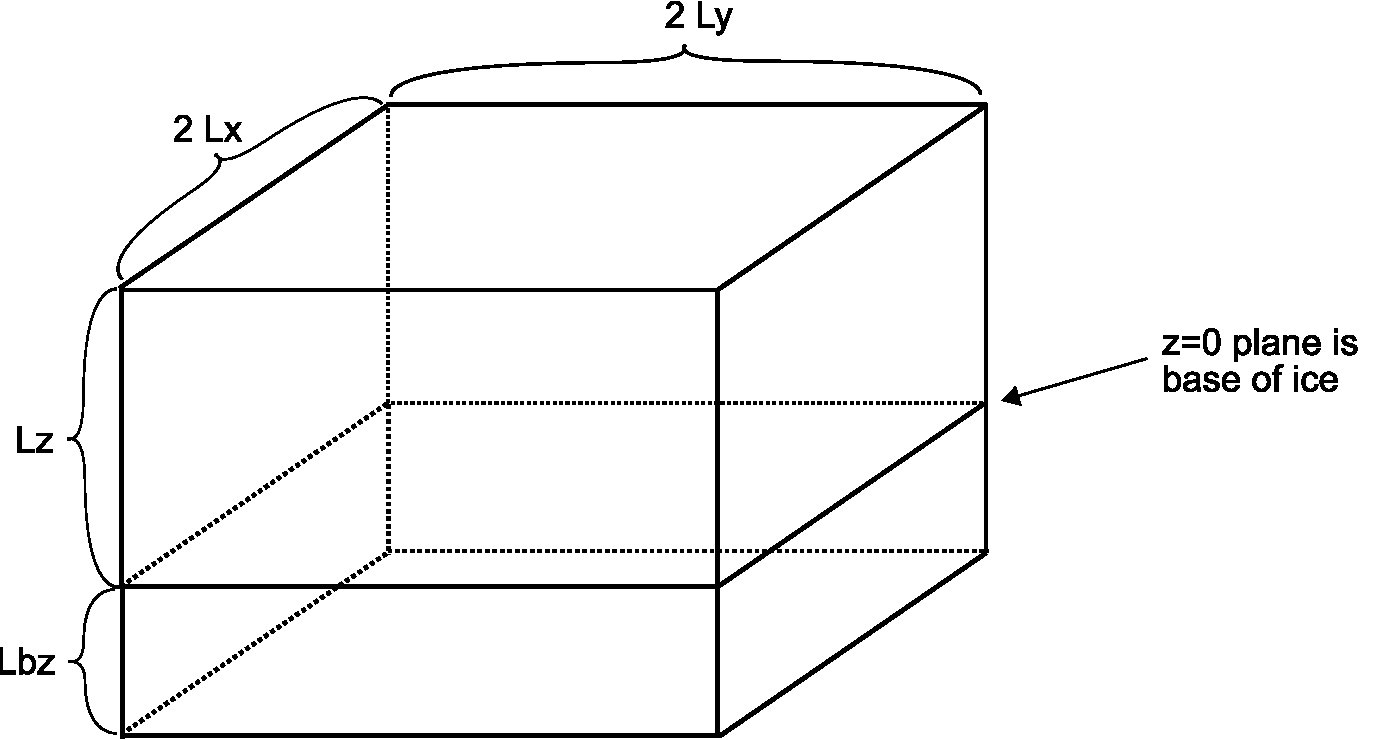
\includegraphics[width=4.0in,keepaspectratio=true]{figs/rectilinearbox}
\caption{PISM's computational box.}
\label{fig:rectilinearbox}
\end{figure}

The extent of the computational box for the ice is directly controlled by the options \t{-Lx}, \t{-Ly}, and \t{-Lz} as described in the Runtime options section.  As noted \t{-Lx} and \t{-Ly} options should include values in kilometers while \t{-Lz} should be in meters.

The PISM grid covering the computational box is equally spaced in each of the three dimensions.  Because of the bedrock extension, the grid of points is described by four numbers, namely the number of grid points in the $x$ direction, the number in the $y$ direction, the number in the $z$ direction within the ice, and the number in the $z$ direction within the bedrock.  These are specified by options \verb|-Mx|, \verb|-My|, \verb|-Mz|, and \verb|-Mbz|, respectively, as described in the Runtime options section.  The defaults for these four values are 61, 61, 31, and 1, respectively.  Note that \verb|Mx|, \verb|My|, \verb|Mz|, and \verb|Mbz| all indicate the number of grid \emph{points}.  Therefore the number of grid \emph{spaces} are, respectively, 60, 60, 30, and 0 (zero) in the default case.  Note that the lowest grid point in a column of ice, that is the one at $z=0$, coincides with the highest grid point in the bedrock.  Also \verb|Mbz| must always be at least one.

The distance \t{Lbz} is controlled by specifying the number \verb|Mbz| of grid points in the bedrock, noting that the vertical spacing \t{dz} is the same within the ice and within the bedrock.  To avoid conflicts, the distance \t{Lbz} should not be set directly by the user.  In particular, $\text{\t{Lbz}}=\text{\t{dz}}\,(\text{\t{Mbz}}-1)$ while $\text{\t{dz}} = \text{\t{Lz}} / (\text{\t{Mz}}-1)$, and so the distance \t{Lbz} into the bedrock is determined by setting \t{Lz}, \t{Mz}, and \t{Mbz}.

One is allowed to specify the grid when PISM is started \emph{without} a pre-existing model state (i.e.~as stored in a NetCDF input file output by PISM).  For instance, a EISMINT II experiment F \cite{EISMINT00} run is

\verb|$  pisms -eisII F -Mx 61 -My 61 -Mz 101 -y 200000 -o foo|

\noindent Note that PISM (i.e.~the executable \verb|pisms|) knows about the size of the computational box appropriate to each of the EISMINT II experiments.

If one initializes PISM from a saved model state then the input model state controls the parameters \t{Mx}, \t{My}, \t{Mz}, and \t{Mbz}.  For instance, the command

\verb|$  pisms -eisII F -if foo.nc -Mz 201 -y 100|

\noindent will give a warning that ``\verb|user option -Mz ignored; value read from file foo.nc|.''  To change the model grid one must explicitly ``regrid'', as described next.

\subsection{Regridding}  It is common to want to interpolate a coarse grid model state onto a finer grid or vice versa.  For example, one might want to do the EISMINT II experiment F as above, producing \verb|foo.nc|, but then interpolate both the ice thickness and the temperature onto a finer grid.  Speaking conceptually, the idea in PISM is that one starts over from the beginning of EISMINT II experiment F on the finer grid, but one extracts the thickness and ice temperature stored in the coarse grid file and interpolates onto the finer grid before proceeding with the actual computation.  The transfer from grid to grid is reasonably general---one can go from coarse to fine or vice versa in each dimension $x,y,z$---but the transfer must always be done by \emph{interpolation} and never \emph{extrapolation}.  (An attempt to do the latter should always produce a PISM error.)

Such ``regridding'' is done using the \verb|-regrid| and \verb|-regrid_vars| commands as in this example:

\verb|$  pisms -eisII F -Mx 101 -My 101 -Mz 201 -y 1000 \|

\verb|     -regrid foo.nc -regrid_vars HT -o bar|

\noindent Note one specifies ``\verb|HT|'' to indicate that the ice thickness and temperature values from the old grid should be interpolated onto the new grid.  See table \ref{tab:regridvar} for the regriddable variables.  Note that one doesn't need to regrid the bed elevation, which is set identically zero as part of the EISMINT II experiment F description, nor the ice surface elevation, which is computed as the bed elevation plus the ice thickness at each time step anyway.

A slightly different use of regridding occurs when ``bootstrapping'' as described in section \ref{sect:real}.  Here it is reasonable to have the sequence of commands, run on 8 processors,
\small
\begin{verbatim}
mpiexec -n 8 pismr -bif_legacy init.nc -Mx 141 -My 141 -Mz 101 -Mbz 21 -gk -e 1.2 \
   -verbose -y 10 -o ant10yr_40km -of n

mpiexec -n 8 pismr -if ant10yr_40km.nc -gk -e 1.2 -no_mass -y 149990 \
   -o ant150k_40km -of n

mpiexec -n 8 pismr -bif_legacy init.nc -Mx 281 -My 281 -Mz 201 -Mbz 41 -gk -e 1.2 \
   -regrid ant150k_40km.nc -regrid_vars TBeL -verbose -y 10 -o ant150k_20km -of n
\end{verbatim}
\normalsize
Here we bootstrap from an incomplete set of data in \verb|init.nc| and smooth the surface for a short 10 year run on a coarseer 40km grid.  Then we do a long simulation to complete 150,000 years on this coarse grid to approximate the temperature and age fields, assuming steady boundary conditions and fixed geometry.  Finally we do a brief 10 year run with evolving geometry on a finer 20km grid, but we go back to the original data for the ice thickness; this last stage involves regridding temperature but not thickness, in particular.


\begin{table}[h]
\caption{Regriddable variables.  Use \texttt{-regrid$\underline{\phantom{b}}$var} with given flag.}\label{tab:regridvar}
\begin{tabular}{@{}llll}\hline
\textbf{Flag} & \textbf{Variable} & \textbf{Comment}\\ \hline
\verb|a| & (net annual) accumulation & \emph{climate data}; usually not regridded \\
\verb|b| & bed elevation & \\
\verb|B| & temperature in bedrock & \\
\verb|e| & age of the ice & \\
\verb|g| & geothermal flux & \emph{climate data}; usually not regridded \\
\verb|H| & thickness & \\
\verb|L| & thickness of basal melt water (stored in till) & \\
\verb|s| & ice surface temperature & \emph{climate data}; usually not regridded\\
\verb|T| & ice temperature & \\
\hline
\normalsize
\end{tabular}
\end{table}

\subsection{Understanding and controlling adaptive time-stepping}  Recall that at each time step we get a summary of the model state using a few numbers.  The format of the summary is
\begin{verbatim}
    $$$$$      YEAR (+    STEP[N$]):     VOL    AREA    MELTF     THICK0     TEMP0
\end{verbatim}
Here we will explain what appears in the `\verb|(+    STEP[N$])|' part of this summary.

\verb|STEP| is the time step just taken by PISM, in model years.  This time step is determined by a somewhat complicated adaptive mechanism.  Note that PISM does each step explicitly when numerically approximating mass conservation in the map-plane.  This requires that PISM have adaptive time-stepping for stability in the shallow ice approximation regions.  Other issues like numerically approximating transport of temperature and age require adaptivity too \cite{BBL}.

Note that most of the time `\verb|N|' will be zero.  The exception is when the option \verb|-tempskip| is used.  If \verb|-tempskip| $M$ is used, then \verb|N| will be at most $M$, and will countdown the mass conservation steps when the adaptive scheme determines that a long temperature/age evolution time step, relative to the diffusity controlled time step for mass conservation, would be allowed.  To see an example, do: 

\verb|$  pismv -test G -Mx 141 -My 141 -Mz 51 -tempskip 4|

Table \ref{tab:adaptiveflag} explains the meaning of the one character adaptive-timestepping flag `\verb|$|'.

\begin{table}[h]
\caption{Meaning of the adaptive time-stepping flag `\texttt{\$}' in `\texttt{(+    STEP[N\$])}'.}\label{tab:adaptiveflag}
\begin{tabular}{@{}llll}\hline
\textbf{Flag} & \textbf{Active adaptive constraint} \\ \hline
\verb|c| & 3D CFL for temperature/age advection \cite{BBL} \\
\verb|d| & diffusivity for SIA mass conservation \cite{BBL} \\
\verb|e| & end of prescribed run time \\
\verb|f| & \verb|-dt_force| set; generally option \verb|-dt_force|, which overrides the adaptive scheme, \\
 & should not be used  \\
\verb|m| & maximum allowed $\Delta t$ applies; set with \verb|-maxdt| \\
\verb|t| & maximum $\Delta t$ was \emph{t}emporarily set by a derived class; e.g.~see effect of deliverables \\
 & \verb|-time|$n$ in \verb|pisms -ismip H \time|$n$ \\
\verb|u| & 2D CFL for mass conservation in Macayeal regions (where mass conservation is \emph{u}pwinded)\\
\hline
\normalsize
\end{tabular}
\end{table}

\subsection{Using signals to observe or stop a running PISM model} \label{subsect:signal}  Ice sheet model runs sometimes take a long time and the state of the run needs checking.  Sometimes they need to be stopped, but with the possibility of restarting.  PISM implements these behaviors using ``signals'' from the POSIX standard, included in Linux and most flavors of Unix.

Here is an example.  Suppose we start a long verification run in the background, with standard out redirected into a file:

\verb|pismv -test G -Mz 101 -y 1e6 -o testGmillion >> log.txt &|

\noindent This run gets a Unix process id (``\verb|pid|''), and we will need that number.  (One can get the \verb|pid| by using the \verb|ps| or \verb|pgrep| utilities.)

If we want to observe the run without stopping it we send the \verb|USR1| signal:

\verb|kill -USR1 8920|

\noindent where ``\verb|8920|'' happened to be the \verb|pid| of the running PISM process.  It happens that we caught the run at year 31871.5 or so because a NetCDF file \verb|pism-31871.495239.nc| is produced.  This intermediate state file can be viewed by \verb|ncview pism-31871.495239.nc|.  Note also that in the standard out log file \verb|log.txt| the lines

\verb|...|

\verb|$vtf  31871.495 (+ 30.84701[0d]):   2.985   1.747    0.000   2997.637   272.236|

\verb|Caught signal SIGUSR1: Writing intermediate file `pism-31871.495239.nc'.|

\verb|$vtf  31904.021 (+ 32.52611[0d]):   2.997   1.747    0.000   2997.641   272.235|

\verb|...|

\noindent appear.

Suppose, on the other hand, that the run needs to be stopped.  One may use the usual interrupt ``\verb|kill 8920|'' or ``\verb|kill -KILL 8920|'' for this process, which is running in the background.  (Foreground processes can be interrupted by Ctrl-C.)  This brutal method stops the process but does not allow it to be restarted because the state is not saved.  If one wants the possibility of restarting then one should used the \verb|TERM| signal, 

\verb|kill -TERM 8920|

\noindent Then the PISM run is stopped, the lines

\verb|Caught signal SIGTERM: exiting early.|

\verb|...|

\verb|Writing model state to file `testGmillion.nc' ... done|

\noindent appear in the log file \verb|log.txt|, and the NetCDF model state file \verb|testGmillion.nc| appears.  Note this file has the original output name.  One can restart and finish by the command

\verb|pismv -test G -if testGmillion.nc -ye 1e6 -o testGmillion_finish >> log_cont.txt &|

\noindent for instance.


\subsection{Using the positive degree-day model}  \label{subsect:pdd}  By default the accumulation map in PISM is treated as net annual accumulation.  If the input data is actually annual snow-fall (measured as ice-equivalent) then one must \emph{compute} the net annual accumulation according to some mode of how much of the snow is melted in each model year.  The mass conservation equation for the ice sheet requires the net annual accumulation, in any case.  Also note that the surface temperature map in PISM is the mean annual surface temperature, so without an additional model or input there is no yearly temperature cycle.

A reasonable method for computing the melting of snowfall, used by PISM, first assumes a sinusoidal temperature cycle over the course of the year.  The amount of summer warming is the difference between the peak of this temperature cycle and its mean.  The default temperature cycle has a constant amount of summer warming.  This constant is specified by \verb|-pdd_summer_warming|.  See section \ref{sect:real} for an alternative model.  Note that the mean temperature is grid-point dependent, as specified by the input surface temperature map (data), so the cycle is different at each map-plane grid location, though the amplitude is the same at each grid point in the default case.  Also, note that, by default, the peak of the cycle occurs on August 1, but we do not believe that the specific date for ``mid-summer'' matters detectably to whole ice sheet dynamics or simulations thereof.

The part of this cycle above $0\!\phantom{|}^\circ \text{C}$ is converted to positive degree days.  This number of positive degree days is multiplied by a coefficient (set by \verb|-pdd_factor_snow|) to compute the amount of snow melted.  Of this melted snow, a fraction (\verb|-pdd_refreeze|) is kept as ice.  This ice, plus all unmelted snow (measured as ice-equivalent) is applied as accumulation, unless the number of positive degree days exceeds that required to melt all of the snow-fall in the year.  In this latter case in which there are excess positive degree days available for melting, the number of excess positive degree days is multiplied by a coefficient (\verb|-pdd_factor_ice|) to compute how much ice is melted, so that net ablation occurs (at the given point).

As an additional feature one may add ``white noise'' to the temperature cycle.  More precisely, a normally-distributed, mean zero random temperature increment is added (or subtracted) from the temperature for each day.  These increments are independent over the days of the year, though of course we only have pseudo-randomness \dots, but they are the same over the whole sheet.  Their standard deviation is controlled by \verb|-pdd_std_dev|.  If one wants runs with repeatable randomness, add the option \verb|-pdd_repeatable|.

As an example of this mechanism, first do

\verb|pisms -eisII A -Mx 61 -My 61 -Mz 101 -y 8000 -o foo|

\noindent to get an ice sheet which is large enough to have spread significantly into the ablation zone.  Next observe how it behaves in a warmer ``climate'' \emph{without} the positive degree day model; note that the peak surface temperature in EISMINT II experiment B is 5.0 degrees warmer than that in experiment A \cite{EISMINT00}:

\verb|pisms -eisII B -if foo.nc -y 40|

\noindent In this 40 year run the ice sheet grows a bit.  Now observe how it behaves with the default positive degree day model:

\verb|pisms -eisII B -if foo.nc -y 40 -pdd|

\noindent Note that this latter run is the same as

\verb|pisms -eisII B -if foo.nc -y 40 -pdd_summer_warming 15.0 -pdd_factor_snow 0.003 \|

\verb|  -pdd_factor_ice 0.008 -pdd_refreeze 0.6 -pdd_std_dev 0.0|

\noindent and that any of these options can be adjusted.

A positive degree day model specific to the Greenland ice sheet is used in section \ref{sect:real}.



\clearpage\newpage
\section{Verification}\label{sect:verif}

\bigskip
\begin{quote}  Two types of errors may be distinguished: modelling errors and numerical errors.  Modelling errors arise from not solving the right equations.  Numerical errors result from not solving the equations right.  The assessment of modelling errors is \emph{validation}, whereas the assessment of numerical errors is called \emph{verification} \dots  Validation makes sense only after verification, otherwise agreement between measured and computed results may well be fortuitous.
\end{quote}
\hfill P.~Wesseling, (2001)  \emph{Principles of Computational Fluid Dynamics}, pp.~560--561 \cite{Wesseling}
\bigskip

``Verification'' is a crucial task for a code as complicated as PISM.  It is the exclusively mathematical and numerical task of checking that the predictions of the numerical code are close to the predictions of the continuum model (the one which the numerical code claims to approximate).  In particular, one compares exact solutions of the continuum model, if available, to their numerical approximations.

See \cite{BLKCB} and \cite{BBL} for discussion of verification issues for the isothermal and thermomechanically coupled shallow ice approximation (SIA), respectively, and for exact solutions to these models.  See \cite{SchoofStream} for an exact solution to the MacAyeal equations for ice streams using a plastic till assumption.

In PISM there is a separate executable \verb|pismv| which is used for verification.  The numerical code which is verified by \verb|pismv| is, however, exactly the same lines of code in exactly the same source files as is run by the non-verification executables \verb|pismr| and \verb|pisms|.  (In technical terms, \verb|pismv| runs a derived class of the core class \verb|IceModel|.  The core class corresponds to \verb|pismr|.)

Table \ref{tab:tests} summarizes the many exact solutions contained within PISM.  Note that all of these exact solutions except tests A and E are solutions of free boundary problems for partial differential equations.

Table \ref{tab:tests_exec} shows how to run them for an example grid, namely a grid recommended for quick execution time.   For serious attempts at verification, however, one must go down a grid refinement path and measure error.  For example, the runs
\begin{quote}\small\begin{verbatim}
pismv -test B -ys 422.45 -y 25000 -Mx 31 -My 31 -Mz 11
pismv -test B -ys 422.45 -y 25000 -Mx 61 -My 61 -Mz 11
pismv -test B -ys 422.45 -y 25000 -Mx 121 -My 121 -Mz 11
pismv -test B -ys 422.45 -y 25000 -Mx 241 -My 241 -Mz 11
\end{verbatim}
\normalsize\end{quote}
verify the basic function of the isothermal shallow ice approximation components of PISM.  The data produced by these four runs appears in figures 7, 8, 9, and 10 of \cite{BLKCB}.  Thereby we see that the isothermal mass conservation scheme does a reasonable job of approximating the evolving surface.

For thermocoupled tests one would refine in three dimensions.  For example, the runs
\begin{quote}\small\begin{verbatim}
pismv -test G -maxdt 10.0 -y 25000 -Mx 61 -My 61 -Mz 61
pismv -test G -maxdt 10.0 -y 25000 -Mx 91 -My 91 -Mz 91
pismv -test G -maxdt 10.0 -y 25000 -Mx 121 -My 121 -Mz 121
pismv -test G -maxdt 10.0 -y 25000 -Mx 181 -My 181 -Mz 181
pismv -test G -maxdt 10.0 -y 25000 -Mx 241 -My 241 -Mz 241
pismv -test G -maxdt 10.0 -y 25000 -Mx 361 -My 361 -Mz 361
\end{verbatim}
\normalsize\end{quote}
produce the error data in figures 13, 14, and 15 of \cite{BBL}.  (Don't do the last couple of these without a supercomputer!  The $361\times 361\times 361$ run involves more than $100$ million unknowns, updated at each of millions of time steps.)

\begin{table}[h]
\caption{Exact solutions for verification.}\label{tab:tests}
\small
\begin{tabular}{@{}llll}\hline
\textbf{Test} & \textbf{Continuum model tested} & \textbf{Comments} & \textbf{Reference} \\ \hline
A & isothermal SIA (mass conservation), steady, &  & \cite{BLKCB} \\
 & flat bed, constant accumulation &  &  \\
B & isothermal SIA, flat bed, zero accum & similarity soln & \cite{BLKCB} \\
C & isothermal SIA, flat bed, growing accum & similarity soln & \cite{BLKCB} \\
D & isothermal SIA, flat bed, oscillating accum & compensatory accum & \cite{BLKCB} \\
E & isothermal SIA; as A &  compensatory accum & \cite{BLKCB} \\
 & but with sliding in a sector &  &  \\
F & thermomechanically coupled SIA (mass &  compensatory accum & \cite{BB,BBL} \\
 & and energy cons.), steady, flat bed & and comp~heating &  \\
G & thermomechanically coupled SIA; as F  & ditto & \cite{BB,BBL} \\
 & but with oscillating accumulation &  &  \\
H & bed deformation coupled with isothermal SIA & joined similarity & \cite{BLKfastearth} \\
I & velocity computation using MacAyeal eqns and plastic till &  & \cite{MacAyeal,SchoofStream} \\
L & isothermal SIA, steady, non-flat bed & numerical ODE soln & \cite{BuelerEquilSheets} \\
\hline
\normalsize
\end{tabular}
\end{table}


\begin{table}[h]
\caption{Running PISM to verify against the exact solutions.}\label{tab:tests_exec}
\small
\begin{tabular}{@{}llll}\hline
\textbf{Test} & \textbf{Example invocation}  \\ \hline
A & \verb|pismv -test A -Mx 61 -My 61 -Mz 11 -y 25000| \\
B & \verb|pismv -test B -Mx 61 -My 61 -Mz 11 -ys 422.45 -y 25000|  \\
C & \verb|pismv -test C -Mx 61 -My 61 -Mz 11 -y 15208.0|  \\
D & \verb|pismv -test D -Mx 61 -My 61 -Mz 11 -y 25000|  \\
E & \verb|pismv -test E -Mx 61 -My 61 -Mz 11 -y 25000|  \\
F & \verb|pismv -test F -Mx 61 -My 61 -Mz 61 -y 25000|  \\
G & \verb|pismv -test G -Mx 61 -My 61 -Mz 61 -y 25000|  \\
H & \verb|pismv -test H -Mx 61 -My 61 -Mz 11 -y 40034 -bed_def_iso| \\
I & \verb|pismv -test I -Mx 5 -My 500 -mv_rtol 1e-6 -ksp_rtol 1e-11| \\
L & \verb|pismv -test L -Mx 61 -My 61 -Mz 31 -y 25000| \\
\hline
\normalsize
\end{tabular}
\end{table}

Note there is a Python script, \verb|verifynow.py|, which runs Tests C, G, and I, and suffices for basic verification of most of the numerical methods in PISM, and is a good test for newly-installed copies of PISM.  It takes two options:\begin{itemize}
\item ``\verb|-n |$N$'' specifies $N$ processors to use (i.e.~\verb|mpiexec -n |$N$ is used if $N>1$); the default is $N=1$;
\item ``\verb|-l |$L$'' specifies $L$ levels of refinement; $L=1,2,3,4,5$ are allowed values and the default is $L=3$.
\end{itemize}
Here is an example run:
\scriptsize\begin{quote}\begin{verbatim}
$ verifynow -n 2 -l 3
  VERIFYNOW using 2 processor(s) and 3 level(s) of refinement
  ++++ verifying isothermal SIA using test C (Mx=My=41,61,81,101,121
       corresponds to dx=dy=50,33.3,25,20,16 km) ++++
  trying "mpiexec -n 2 pismv -test C -Mx 41 -My 41 -Mz 31 -y 15208.0 -verbose 1"
  finished in 10.8591 seconds; reported numerical errors as follows:
    |Actual ERRORS evaluated at final time (relative to exact solution):
    |geometry  :  prcntVOL  prcntAREA       maxH       avH   relmaxETA    domeH
    |               0.7189    12.6255   250.0035   12.0155    0.019159  10.0400
  trying "mpiexec -n 2 pismv -test C -Mx 61 -My 61 -Mz 31 -y 15208.0 -verbose 1"
  finished in 36.7092 seconds; reported numerical errors as follows:
    |Actual ERRORS evaluated at final time (relative to exact solution):
    |geometry  :  prcntVOL  prcntAREA       maxH       avH   relmaxETA    domeH
    |               0.1268     6.5122   224.3489    7.1291    0.012296   4.4014
  trying "mpiexec -n 2 pismv -test C -Mx 81 -My 81 -Mz 31 -y 15208.0 -verbose 1"
  finished in 112.6159 seconds; reported numerical errors as follows:
    |Actual ERRORS evaluated at final time (relative to exact solution):
    |geometry  :  prcntVOL  prcntAREA       maxH       avH   relmaxETA    domeH
    |               0.1970     5.5536   194.2413    4.1316    0.008131   2.1267
  ++++ verifying plastic till ice stream using test I (My=49,193,769,3073,12289
       corresponds to dy=5000,1250,312.5,78.13,19.53 m) ++++
  trying "mpiexec -n 2 pismv -test I -My 49 -Mx 5 -mv_rtol 5e-07 -ksp_rtol 1e-12 -verbose 1"
  finished in  0.9357 seconds; reported numerical errors as follows:
    |Actual ERRORS in velocity relative to exact solution:
    |      maxvector   avvector  prcntavvec      maxu      maxv       avu       avv
    |        23.3329    7.69421     0.98956   23.3329    0.0000    7.6942    0.0000
  trying "mpiexec -n 2 pismv -test I -My 193 -Mx 5 -mv_rtol 5e-07 -ksp_rtol 1e-12 -verbose 1"
  finished in  3.8574 seconds; reported numerical errors as follows:
    |Actual ERRORS in velocity relative to exact solution:
    |      maxvector   avvector  prcntavvec      maxu      maxv       avu       avv
    |         1.3246    0.44147     0.05678    1.3246    0.0000    0.4415    0.0000
  trying "mpiexec -n 2 pismv -test I -My 769 -Mx 5 -mv_rtol 5e-07 -ksp_rtol 1e-12 -verbose 1"
  finished in 16.2246 seconds; reported numerical errors as follows:
    |Actual ERRORS in velocity relative to exact solution:
    |      maxvector   avvector  prcntavvec      maxu      maxv       avu       avv
    |         0.0923    0.03117     0.00401    0.0923    0.0000    0.0312    0.0000
  ++++ verifying thermocoupled SIA using test G (Mx=My=Mz=61,91,121,181,241
       corresponds to dx=dy=30,20,15,10,7.5 km and dz=66.7,44.4,33.3,22.2,16.7 m) ++++
  trying "mpiexec -n 2 pismv -test G -Mx 61 -My 61 -Mz 61 -y 25000.0 -verbose 1"
  finished in 119.0501 seconds; reported numerical errors as follows:
    |Actual ERRORS evaluated at final time (relative to exact solution):
    |geometry  :  prcntVOL  prcntAREA       maxH       avH   relmaxETA    domeH
    |               2.1076     0.0000    64.3642   19.5506    0.017980   2.8224
    |base temps:        maxT         avT      domeT
    |               1.533177    0.471904   0.069055
  trying "mpiexec -n 2 pismv -test G -Mx 91 -My 91 -Mz 91 -y 25000.0 -verbose 1"
  finished in 878.9009 seconds; reported numerical errors as follows:
    |Actual ERRORS evaluated at final time (relative to exact solution):
    |geometry  :  prcntVOL  prcntAREA       maxH       avH   relmaxETA    domeH
    |               0.9508     0.0000    29.7903    9.0329    0.007974   0.0095
    |base temps:        maxT         avT      domeT
    |               0.962611    0.238721   0.025394
  trying "mpiexec -n 2 pismv -test G -Mx 121 -My 121 -Mz 121 -y 25000.0 -verbose 1"
  finished in 3777.5895 seconds; reported numerical errors as follows:
    |Actual ERRORS evaluated at final time (relative to exact solution):
    |geometry  :  prcntVOL  prcntAREA       maxH       avH   relmaxETA    domeH
    |               0.5216     0.0000    28.3494    4.9974    0.004423   0.8286
    |base temps:        maxT         avT      domeT
    |               0.781534    0.140056   0.003918
\end{verbatim}
\end{quote}\normalsize


\clearpage\newpage
\section{Simplified geometry experiments}\label{sect:simp}

\subsection{Historical note}  There have been at least three stages of ice sheet model intercomparisons based on simplified geometry experiments since the early 1990s.

EISMINT I \cite{EISMINT96} was the first of these and involved only the isothermal shallow ice approximation (SIA).  ``EISMINT'' stands for European Ice Sheet Modeling INiTiative.  Both fixed margin and moving margin experiments were performed in EISMINT I, and various conclusions were drawn about the several numerical schemes used in the intercomparison.  

EISMINT I is, however, superceded by \emph{verification} using the full variety of exact solutions to the isothermal SIA.  The reasons why EISMINT I can be fully replaced by verification are described in \cite{BLKCB}.  The ``rediscovery'', since EISMINT I, of the very useful Halfar similarity solution with zero accumulation \cite{Halfar83} is a particular reason why the ``moving margin'' experiment in EISMINT I is, roughly speaking, irrelevant.  For this reason there has been no attempt to support the EISMINT I experiments in PISM.  (On the other hand, EISMINT I is a perfectly reasonable task for PISM.  It is strictly easier to perform the EISMINT I experiments than the verification relative to tests A, B, C, D, and E described in the previous section.  But one learns \emph{much} more about numerical performance through verification with exact solutions, and in the isothermal flat base case considered in EISMINT I, the selection of exact solutions is copious.)

EISMINT II \cite{EISMINT00} was both a more significant, and certainly more controversial, intercomparison.  It clearly pointed out interesting and surprising properties of the thermocoupled SIA.  Here is not the place for a discussion of the interpretations which have followed the EISMINT II results, but references \cite{BBL,Hindmarsh04,Hindmarsh06,PayneBaldwin,SaitoEISMINT} each interpret the EISMINT II experiments and/or describe attempts to add more complete physical models to ``fix'' the perceived shortfalls of ice sheet models.   (I.e.~shortfalls revealed by the EISMINT II results and their interpretations.)  PISM has built-in support for reproduction of all of the EISMINT II experiments; these are described in the next subsection.

The ISMIP round of intercomparisons are ongoing at the time of this writing (2007); ``ISMIP'' stands for Ice Sheet Model Intercomparison Project.  At this time there are three components of ISMIP namely HOM = Higher Order Models, HEINO = Heinrich Event INtercOmparison, and POLICE = POLar ICE sheet modelss.  None of these are completed and published and the last is still in early planning.  

Of these ISMIP experiments, PISM currently only supports HEINO, but the results from PISM for HEINO are not regarded by the PISM authors as meaningful.  The point is that we believe the continuum problem described by HEINO to be not-easily-approximateable, regardless of the details of the numerical schemes.  (Feel free to write to \verb|ffelb@uaf.edu| on this topic, of course.)

Again as of July 2007, the PISM authors plan to participate in ISMIP-POLICE and an upcoming Marine Ice Sheet Intercomparison exercise.

\subsection{EISMINT II in PISM}  There are seven experiments described in the EISMINT II writeup \cite{EISMINT00}. They are labeled A, B, C, D, F, G, and H.  As specified in the writeup, the common features of all of these experiments are:\begin{itemize}
\item runs are of 200,000 years, with no prescribed time step;
\item runs are on a prescribed $61\times 61$ horizontal grid (but, as usual, the grid and the length of the run are command line options in PISM so PISM can easily run the same experiments on a refined grid);
\item the boundary conditions always have angular symmetry around the center of the grid;
\item the bed is always flat and does not move (so the effects of isostasy were ignored throughout);
\item the temperature in the bedrock is not modelled;
\item only shallow ice approximation physics is included;
\item thermodynamics is included in that the temperature of ice is controlled by conservation of energy;
\item thermomechanical coupling is included, both because of the temperature dependence of the softness of the ice, \emph{and} through the strain-heating (dissipation-heating) term in the conservation of energy equation;
\item the ice is \emph{cold} and not \emph{polythermal} \cite{Greve}; and finally
\item though basal melt rates may be computed diagnostically, they do not contribute to the thermomechanical evolution of the ice sheet.
\end{itemize}
The experiments differ from each other in their various combinations of surface temperature and accumulation parameterizations.  Also, experiments H and G involve basal sliding, while the others don't.  Some experiments start with zero ice (A,F,G,H) while some start from the end state of other experiments.  In particular, experiments B, C, and D start from the final state of experiment A.

The vertical grid is not specified in the EISMINT II writeup.  It seems that good simulation of the complex thermomechanically coupled conditions near the base of the ice requires relatively fine resolution there.  Because PISM (currently) has an equally-spaced grid, we recommend the use of about 200 vertical levels.

Thus a reasonable experiment A run on four processors is

\verb|mpiexec -n 4 pisms -eisII A -Mx 61 -My 61 -Mz 201 -y 200000 -o eisIIA|

\noindent Note that once the above run is completed, which might take an hour or two on the four processors in this case, something like

\verb|mpiexec -n 4 pisms -eisII A -if eisIIA.nc -d HTcf -display :0|

\noindent will give a quick view of thickness, basal temperature, the vertically-integrated horizontal speed of the ice, and the residual rate of change of the thickness at the final state.  A more complete view of the final state using \verb|ncview| is of course worthwhile.

Table \ref{tab:eisII} shows how the other EISMINT II experiments can be done in PISM.  As noted, experiments B,C,D start from the saved state of experiment A.

\begin{table}[h]
\caption{Running the EISMINT II experiments in PISM; the command is ``\t{pisms}'' plus these options.}\label{tab:eisII}
\small
\begin{tabular}{@{}llll}\hline
\textbf{Command: ``\t{pisms}'' $+$} & \textbf{Relation to experiment A} \\ \hline
\verb|-eisII A -Mx 61 -My 61 -Mz 201 -y 2e5 -o eisIIA| & \\
\verb|-eisII B -if eisIIA.nc -y 2e5 -o eisIIB| & warmer \\
\verb|-eisII C -if eisIIA.nc -y 200000 -o eisIIC| & less snow \\
\verb|-eisII D -if eisIIA.nc -y 200000 -o eisIID| & smaller area of accumulation \\
\verb|-eisII F -Mx 61 -My 61 -Mz 201 -y 200000 -o eisIIF| & colder; famous spokes \cite{BBL} \\
\verb|-eisII G -Mx 61 -My 61 -Mz 201 -y 200000 -o eisIIG| & sliding (regardless of temperature) \\
\verb|-eisII H -Mx 61 -My 61 -Mz 201 -y 200000 -o eisIIH| & melt-temperature activated sliding \\
\hline\normalsize
\end{tabular}\end{table}

The EISMINT II experiments can be run with various modifications of the default settings.  Certainly the grid can be refined.  For instance, a twice as fine grid in the horizontal is ``\t{-Mx 121 -My 121}''.  Table \ref{tab:eisIIoptions} lists the optional settings which are particular to the EISMINT II experiments; these options will only work if option ``\t{-eisII ?}'' is also set.

\begin{table}[h]
\caption{Changing the default settings for the EISMINT II experiments in PISM.}\label{tab:eisIIoptions}
\small
\begin{tabular}{@{}llll}\hline
\textbf{Option} & \textbf{Default values [expers]} & \textbf{Units} & \textbf{Meaning} \\ \hline
\verb|-Mmax| & 0.5 [ABDFGH], 0.25 [C] & m$/$a & max value of accumulation rate \\
\verb|-Rel| & 450 [ABFGH], 425 [CD] & km & radial distance to equilibrium line \\
\verb|-Sb| & $10^{-2}$ [\emph{all}] & (m/a)/km & radial gradient of accumulation rate \\
\verb|-ST| & $1.67 \times 10^{-2}$ [\emph{all}] & K/km & radial gradient of surface temperature\\
\verb|-Tmin| & 238.15 [ACDGH], 243.15[B], 223.15[F] & K & max of surface temperature \\ \hline
\verb|-Lz| & 4500 [A], 4000 [BCD], 5000 [F], 3000 [G] & m & height of the computational box \\
\hline\normalsize
\end{tabular}\end{table}

Note that in PISM the height \verb|Lz| of the computational box is fixed at the beginning of the run.  On the other hand, changing the boundary conditions of the flow, as for instance by setting option \verb|-Mmax| to a larger than default value (see table \ref{tab:eisIIoptions}), may cause the ice sheet to thicken above the \verb|Lz| height.  If the ice grows above the height of the computational box then a ``\verb|Vertical grid exceeded!|'' or ``\verb|thickness overflow in SIA velocity: ks>Mz!|'' error occurs.  This can be fixed by remedied by restarting with a larger value for option \verb|-Lz|.


\begin{comment}
\subsection{ISMIP-HEINO in PISM}  The goal of the ISMIP-HEINO intercomparison is to evaluate the degree to which the thermomechanically coupled shallow ice approximation with basal sliding is a model for the surge behavior of the Laurentide ice sheet which is believed to have caused the ``Heinrich events'' described in [CITE HEINRICH].  Further information about HEINO, including the intercomparison description [URL FOR HEINO PDF] can be found at \url{http://www.pik-potsdam.de/~calov/heino.html}.

HEINO involves eight different runs of 200,000 years on a prescribed $81\times 81$ grid in the horizontal.  As in EISMINT II there is no prescription of vertical grid.  During the entirety of each run certain integrated quantities (area, melted base area, etc.) and other quantities measured at prescribed basal points must be reported at each year into ASCII files with \verb|.dat| extensions.  During the last 50,000 years of each of the eight runs, a map-plane (``planform'') dump of other quantities must be made to additional \verb|.dat| ASCII files.  These latter dumps must be made at the time of maximum and minimum extents of various quantities and the only way to determine the time of maximum/minimum extents is to complete the 200,000 year runs, determine the times of maximum and minimums, and then rerun the last 50,000 years from the saved state at 150,000 years.  See the intercomparison description [CITE URL for PDF].

PISM handles all the difficult details of the procedures described in the previous paragraph, but it is important for the user to have a sense for what is supposed to be reported.

HEINO is a relatively expensive intercomparison in terms of computer time.  For this reason use of a multiprocessor machine is recommended though not essential.  If the intercomparison participant's initials were X.~Y.~Z.~then a HEINO run ST is the recipe

\verb|mpiexec -n 8 pisms -ismip H -run ST -Mx 81 -My 81 -Mz 281 \|

\verb|    -y 150000 -dat_prefix XYZ_START -o XYZ_ST_150k|

\verb|mpiexec -n 8 pisms -ismip H -run ST -if XYZ_ST_150k.nc \|

\verb|    -y 50000 -dat_prefix XYZ_END -o XYZ_ST_200k|

[use Matlab to determine max/min]

\verb|mpiexec -n 8 pisms -ismip H -run ST -if XYZ_ST_150k.nc \|

\verb|    -y 50000 -time1 -time2 -time3 -time4 -dat_prefix XYZ_RERUN|

\verb|~/pism/test/heinocatdat.sh XYZ_ST_??? ...|

\verb|~/pism/test/renames.sh | [rename planform files?]

\noindent At the end of the above recipe the files [list] should appear.

\begin{table}[h]
\caption{Options used in running ISMIP-HEINO in PISM.}\label{tab:heinooptions}
\small
\begin{tabular}{@{}llll}\hline
\textbf{Option} & \textbf{Default value(s)} & \textbf{Comments} \\ \hline
\verb|-| & & \\
\verb|-| & & \\
\verb|-dat_prefix| & \verb|PISM| & put initials here \\
\verb|-| & & \\
\verb|-ismip| & \verb|H| & only HEINO implemented for now \\
\verb|-| & & \\
\verb|-| & & \\
\verb|-| & & \\
\hline\normalsize
\end{tabular}\end{table}
\end{comment}


\clearpage\newpage
\section{Validation}\label{sect:valid}

\subsection{Validation of ice shelf numerics relative to Ross ice shelf data}  In \cite{MacAyealetal} a well-known validation of several ice shelf numerical models was performed relative to data from RIGGS (= Ross Ice shelf Geophysical and Glaciological Survey) \cite{RIGGS1,RIGGS2}.  The RIGGS data was acquired in the period 1973--1978 by classical surveying techniques.   This validation was part of the EISMINT I  series of intercomparisons; the intercomparison reported in \cite{EISMINT96} was also in that series.

Performing this validation requires data from the website \url{http://homepages.vub.ac.be/~phuybrec/eismint/iceshelf.html}.  In particular, these files must be downloaded:
\begin{itemize}
\item \verb|111by147Grid.dat|
\item \verb|kbc.dat|
\item \verb|inlets.dat|
\end{itemize}
For easiest use, create the directory \verb|pism/eisROSS|, and put these three \verb|.dat| files there.

Note that the data is for a fixed $6.822$km grid and \emph{this is an unusual use of PISM in that the grid cannot be adjusted}.

Run this validation with \verb|pisms -ross|.  The next several examples are suggested methods for performing the validation.  Note that this Ross ice shelf validation can only be run using a single processor; ``\verb|mpiexec -n |$N$\verb| pisms -ross|'' generates an error.  Table \ref{tab:rossoptions} shows options available for this validation; note these options are also described in the Runtime Options section above.

\bigskip
\noindent\textbf{Example 1}.  Basic run with all info displayed: 

\verb|pisms -ross -d cnmu -pause 10 -showobsvel -verbose|

\noindent Note $\bar B = 2.22 \times 10^8$ versus $\bar B = 1.9 \times 10^8$ as in \cite{MacAyealetal}.  Files \verb|pism/eisROSS/111by147Grid.dat|, \verb|pism/eisROSS/kbc.dat|, and \verb|pism/eisROSS/inlets.dat| must be present (though \verb|-prefix| can be used if they are at a different location).

\bigskip
\noindent\textbf{Example 2}.  Do same as above but save \Matlab results:

\verb|pisms -ross -verbose -o ross_2p22e8 -of m|

\noindent Note there is no graphical display.  The resulting file \verb|ross_2p22e8.m| can be run in \Matlab as a script.

The files \verb|README.rossPISM|, \verb|riggs_ELBclean.dat|, and \verb|ross_plot.m| in subdirectory \verb|pism/test/ross/| can be used to produce $\chi^2$ statistic relative to RIGGS data \cite{MacAyealetal}, and to give a nice picture.  In particular, once the above PISM run finishes and \verb|ross_2p22e8.m| is saved in a location on the \Matlab path, and once \verb|pism/test/ross/| is added to the \Matlab path, one can enter these commands at the \Matlab prompt:
\small\begin{verbatim}
>> ross_2p22e8
...
>> ross_plot
ChiSqr =
       3043.7
max_computed_speed =
       1129.9
\end{verbatim}
\normalsize
These results compare well to those in table 1 of \cite{MacAyealetal}.  The figures \ref{fig:rossscatter} and \ref{fig:rossvelocities} below are also produced.

\begin{figure}[ht]
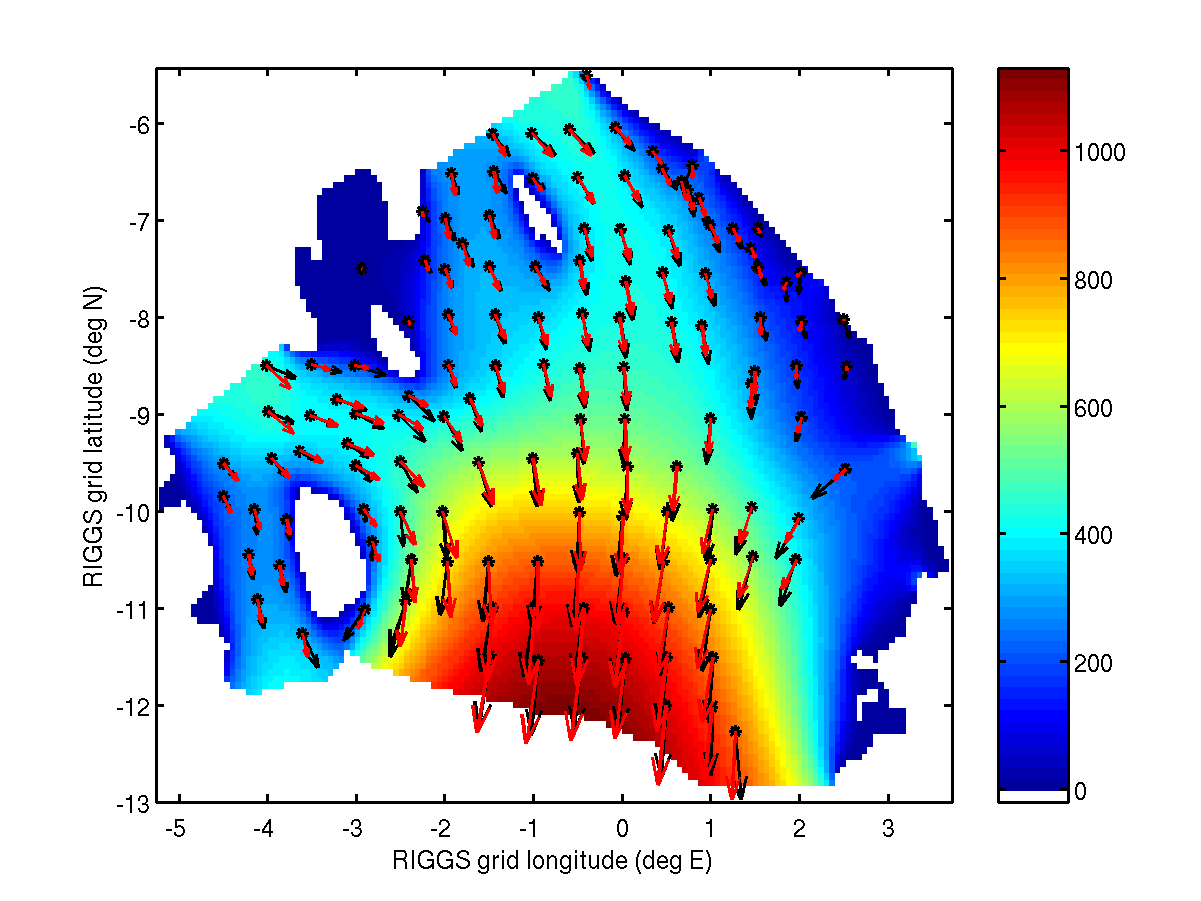
\includegraphics[width=4.5in,keepaspectratio=true]{figs/rossvelocities}
\caption{Color is speed in m/a.  Arrows are observed (black) and computed (red) velocities at RIGGS points.}
\label{fig:rossvelocities}
\end{figure}

\begin{figure}[ht]
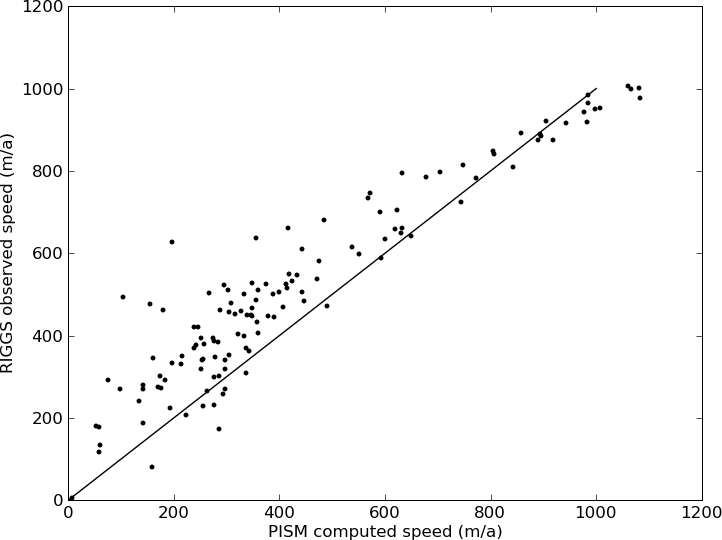
\includegraphics[width=3.5in,keepaspectratio=true]{figs/rossscatter}
\caption{Comparison between modelled and observed velocities at RIGGS points; compare figure 2  in \cite{MacAyealetal}.}
\label{fig:rossscatter}
\end{figure}

\bigskip
\noindent\textbf{Example 3}.  Same as \textbf{Example 1}, but asking for a lot more accuracy:

\verb|pisms -ross -d cnmu -pause 10 -showobsvel -verbose \|

\verb|  -mv_rtol 1e-7 -ksp_rtol 1e-10|

\noindent In fact one gets nearly the same result,  which suggests the default tolerances (\verb|-mv_rtol 1e-4| \verb|-ksp_rtol 1e-6|) suffice.

\bigskip
\noindent\textbf{Example 4}.  Tune across range of values of $\bar B$, including \cite{MacAyealetal}
value.

\verb|pisms -ross -verbose -tune 1.7e8,1e7,2.4e8|

\noindent One sees why $\bar B = 2.22\times 10^8$ is used as default value by PISM.

\small
\begin{table}[h]
\caption{Options available and/or recommended when validating using EISMINT Ross data; run with \texttt{obj/pisms -ross}.}\label{tab:rossoptions}
\begin{tabular}{@{}llll}\hline
\textbf{Option} & \textbf{Explanation/Comments} \\ \hline
  \verb|-d cnmu| &       most useful way to see what is going on \\
  \verb|-if foo| &       NOT allowed!  (there is no way to initialize from an input file) \\
  \verb|-Mx|, \verb|-My| & do not adjust \\
  \verb|-o foo -of m| &  writes data to foo.m; note that an output file \verb|foo.nc| (from \verb|-o foo -of n|) may also be useful \\
  \verb|-pause N| &      pause for N seconds when refreshing viewers \\
  \verb|-prefix foo| &   looks for files \verb|111by147Grid.dat|, \verb|kbc.dat|, and 
                \verb|inlets.dat| in \verb|pism/foo/|; \\
    & files are from \url{http://homepages.vub.ac.be/~phuybrec/eismint/iceshelf.html}; \\
    & by default PISM looks in directory \verb|pism/eisROSS/| if \verb|-prefix foo| is not specified \\
  \verb|-ross| &         to start the Ross validation; note it works only under executable \verb|pisms| \\
  \verb|-showobsvel| &   shows observed (but interpolated) speeds from \verb|111by147Grid.dat| \\
  \verb|-tune x,y,z| &   run through $\bar B$=\verb|x:y:z| (\Matlab syntax), that is, 
                $\bar B = x, x+y, x+2y, \dots$, \\
    & $x+Ny=z$ as hardness parameters; note no spaces in ``\verb|x,y,z|'' \\
  \verb|-verbose| &      shows information on nonlinear iteration and Krylov solve \\
  \verb|-verbose 5| &      shows, in particular, which lines were ignored during reads of \verb|???.dat| files, \\
    & and parameters related to solving the ice shelf equations \\
\hline
\end{tabular}
\end{table}
\normalsize


\clearpage\newpage
\section{Realistic ice sheet modelling}\label{sect:real}
\subsection{Obtaining Greenland Data}  As stated earlier, real data is not something we can freely distribute under the GNU Public License.  Thus, this section describes the use of Python scripts (\verb|eis_green.py| and \verb|eis_core.py|) to convert the EISMINT Greenland data into NetCDF files useable by PISM.

The Python scripts \verb|eis_green.py| and \verb|eis_core.py| can be found in the \verb|pism/test| directory.  In order to use the scripts, you must have the following on your system:\begin{itemize}
 \item The data files \verb|grid20-EISMINT| (or \verb|grid40-EISMINT|), \verb|suaq20-EISMINT| (or \verb|suaq40-EISMINT|), 
 \verb|specmap.017|, and \verb|sum89-92-ss09-50yr.stp| from \url{http://homepages.vub.ac.be/~phuybrec/eismint/greenland.html}.
 \item Installations of Numpy (\url{http://numpy.scipy.org/}) and pycdf (\url{http://pysclint.sourceforge.net/pycdf/}).
\end{itemize}

\noindent The script \verb|eis_green.py| has one, optional command line argument (\verb|-g|). This argument takes one value (should be 20 or 40) which is used to identify if you are using the 20km or 40km gridded data (\verb|grid20-EISMINT| and \verb|suaq20-EISMINT| or \verb|grid40-EISMINT| and \verb|suaq40-EISMINT|). By default, \verb|grid20-EISMINT| and \verb|suaq20-EISMINT| will be used. As for the \verb|eis_core.py| script, there are two options, \verb|-s| and \verb|-t|, that are used to specify how to interpolate the change in sea level data and the change in temperature data respectively. The three types of interpolation currently implemented in \verb|pgrn| are ``linear'', ``constant\_piecewise\_forward'', and ``constant\_piecewise\_backward''.  Now, from a directory with the EISMINT data files, run:

\small\begin{quote}\begin{verbatim}
$  eis_green.py -g 20
\end{verbatim}
\end{quote}\normalsize

and

\small\begin{quote}\begin{verbatim}
$  eis_core.py -t constant_piecewise_backward -s linear
\end{verbatim}
\end{quote}\normalsize

\noindent As a result, two NetCDF files named \verb|eis_green20.nc| (or \verb|eis_green40.nc|) and \verb|eis_core.nc| will be created in the same directory.  The NetCDF file \verb|eis_green20.nc| is the EISMINT Greenland data consisting of values for latitude (\verb|lat|), longitude (\verb|lon|), surface altitude (\verb|S|), bedrock altitude (\verb|b|), and ice thickness (\verb|H|).  These values can easily be viewed using Ncview (\url{http://meteora.ucsd.edu/~pierce/ncview_home_page.html}) with the command:

\small\begin{quote}\begin{verbatim}
$  ncview eis_green.nc
\end{verbatim}
\end{quote}\normalsize

\noindent In order to perform somewhat of a checksum on the \verb|eis_green.nc|, the NCO tools (\url{http://nco.sourceforge.net/}) can be used.  The following command creates a new NetCDF file named \verb|eis_green_check.nc| with a variable called \verb|check|:

\small\begin{quote}\begin{verbatim}
$  ncap -O -vs "check=S-(H+b)" eis_green.nc eis_green_check.nc
\end{verbatim}
\end{quote}\normalsize

\noindent This variable holds the difference of \verb|S| and $\verb|b|+\verb|H|$.  Viewing this variable will show that \verb|S| is within 1 meter of $\verb|b|+\verb|H|$ and is considered to be redundant.  Thus, this data will be ignored.

It also should be noted that bed elevation (\verb|b|) contains a missing value attribute of $0.0$. When viewing this data in Ncview, these values will show as white spots. If these missing values are left in, sharp formations may appear after some time in PISM. Thus, it might be useful to `smooth' the data. This can be done with another script named \verb|fill_missing.py|. To use this script, the following command can be run:

\small\begin{quote}\begin{verbatim}
$  fill_missing.py -i eis_green.nc -v b
\end{verbatim}
\end{quote}\normalsize

\noindent Here, \verb|eis_green.nc| is the input file, and \verb|b| is the variable with missing values. The script will look for an attribute named \verb|missing_value| and fill in the missing values according to the averages of its neighbors. Multiple variables can be fixed at the same time by separating the variable names by commas (e.g. \verb|fill_missing.py -i data.nc -v b,H,Ts|). The only requirement is that each variable has an attribute named \verb|missing_value|.

The file \verb|eis_core.nc| contains the GRIP data used for the climate forcing options which will be explained later.

In addition to getting the EISMINT data into a NetCDF format and filling missing values, there is an issue with Ellesmere Island. Ellesmere Island is very close to Greenland, and so it is possible for the ice sheet to jump over onto to it. Since we don't know much about ice sheets on Ellesmere Island, we want to prevent this from happening. So within the \verb|pgrn| derived class, any bedrock above sealevel northwest of the line connecting $(68.18^\circ E, 80.1^\circ N)$ and $(62^\circ E, 82.24^\circ N)$ was removed (the same applies to anything southeast of $(30^\circ E, 67^\circ N)$ due to the tip of Iceland).

\subsection{Bootstrapping EISMINT Greenland Data}  Once the EISMINT Greenland data is obtained and formatted properly, bootstrapping can begin.  A very simple run is shown below using the \verb|-verbose| option in order to show what is happening.

\small\begin{quote}\begin{verbatim}
$  pgrn -bif eis_green20.nc -Mx 83 -My 141 -y 0 -o grn0y_20km -verbose
   PGRN (EISMINT Greenland mode)
   bootstrapping by PISM default method from file test/eis_green20.nc
     using default value Lz=5000.000000 for vertical extent of computational box for ice
     WARNING: ignoring values found for surface elevation h and using h = b + H
     WARNING: surface temperature Ts not found. Filling in with default value: 263.150000
     WARNING: geothermal flux ghf not found. Filling in with default value: 0.042000
     uplift not found. Filling with zero
     determining mask by floating criterion; grounded ice marked as SIA (=1)
     setting accumulation in ice shelf-free ocean to default value -20.000000
    Hmelt not found. Filling with zero
   bootstrapping done
     [computational box for ice: ( 1640.00 km) x ( 2800.00 km) x ( 5000.00 m)]
     [grid cell dimensions     : (   20.00 km) x (   20.00 km) x (  166.67 m)]
   ...
   done with run ... 
   Writing model state to file `grn0y_20km.nc' ... done.

\end{verbatim}
\end{quote}\normalsize

\noindent Since the EISMINT Greenland data does not contain certain variables necessary to run PISM, this bootstrapping mode fills in several default values. For instance, the variables \verb|Ts|, \verb|ghf|, \verb|uplift|, and \verb|Hmelt| were not found in \verb|eis_green.nc|. Thus, these variables were filled with default \verb|263.15|, \verb|0.042|, \verb|0|, and \verb|0| respectively. Also, recall that the EISMINT Greenland data had redundant surface elevation (\verb|h|) values. When bootstrapping, \verb|h| is ignored and PISM uses the sum of bed elevation and ice thickness (\verb|Ignoring values found for h and using h = b + H|).

\subsection{Running Greenland Experiments Using Bootstrapped Data}
There are several experiments that can be run using command line arguments with \verb|pgrn|. The first experiment is a steady state run using the parameters specified in the EISMINT Intercomparison (-ssl2). This experiment is intended to be run until the model reaches a ``steady state'' (less than a .01\% change in volume in 10,000 years). To run this experiment, there is a script that automates the process so that it is not necessary to manually check the changes in volume . This script is called \verb|ssl2_expr.py| and can be found in the \verb|pism/test| directory. When run, it will continue, saving states every 10,000 years, until the change in volume is less than .01\% between 10,000 year runs. It can take two options at the command line. the first is \verb|-n| which is used to specify the number of processors to be used, and the second is \verb|--ssl3| which is used to tell the script to run a steady state run under a different flow law (Goldsby-Kohlstedt). An example use of \verb|ssl2_expr.py| to run the first steady state experiment on 8 processors is as follows:

\small\begin{quote}\begin{verbatim}
$  ssl2_expr.py -n 8
\end{verbatim}
\end{quote}\normalsize

The next experiment is intended to be carried out after the completion of the first steady state run using the steady model state. The main focus here is the option \verb|-forcing| which uses the GRIP data in \verb|eis_core.nc| to somewhat force the climate. Before every time step, \verb|pgrn| adds in a change to the surface temperature and sea level in order to simulate part of a global climate system, which is specified in \verb|eis_core.nc| and interpolated between years according to the options chosen when \verb|eis_core.py| was run. The data in \verb|eis_core.nc| goes about 250,000 years into the past. Therefore, it is necessary to manually set the year into the past when running \verb|pgrn|. To do this, the option \verb|-ys| is used. This experiment can be run using the following command:

\small\begin{quote}\begin{verbatim}
$  pgrn -ccl3 -if green20_SSL3.nc -forcing eis_core.nc -ys -249900 \
     -ye 0 -o green20_CCL3_y0
\end{verbatim}
\end{quote}\normalsize

\noindent The EISMINT Intercomparison also calls to run for another 500 years with $\bigtriangleup$T and $\bigtriangleup$Sea set to zero. If \verb|pgrn| is run beyond the times in the climate forcing data, this is exactly what it will do. So the rest of the experiment can be run using the following command:

\small\begin{quote}\begin{verbatim}
$  pgrn -ccl3 -if green20_CCL3_y0.nc -forcing eis_core.nc -y 500 \
     -o green20_CCL3_y500
\end{verbatim}
\end{quote}\normalsize

\noindent The last experiment (Greenhouse Warming) described in the EISMINT Intercomparison uses the model state obtained for present day (1989). From the commands before, this is file \verb|green20_CCL3_y0.nc|. The Greenhouse Warming experiment (option \verb|-gwl3|) is intended to be run for 500 years with the temperature increasing by $0.035^\circ C/$year for the first 80 years, then at a rate of $0.0017^\circ C/$year for the last 420 years. The following command will run this experiment:

\small\begin{quote}\begin{verbatim}
$  pgrn -gwl3 -if green20_CCL3_y0.nc -y 500 -o green20_GWL3
\end{verbatim}
\end{quote}\normalsize


\clearpage\newpage
\section{Inside PISM: overviews of models, schemes, and sources}\label{sect:over}

\subsection{The continuum models in PISM}  Significant features of the continuum model approximated by the PISM include:\begin{itemize}
\item The inland ice sheet is modeled with the thermocoupled shallow ice approximation equations \cite{Fowler}, and some temperature-activated basal sliding is allowed.
\item Ice shelves and ice streams are modeled by shallow equations which describe flow by longitudinal strain rates and basal sliding.  These equations are different from the shallow ice approximation.  In shelves and streams the velocities are independent of depth within the ice.  The equations were originally established for ice shelves \cite{Morland,MorlandZainuddin,MacAyealetal}.  They were adapted for ice streams, as ``dragging ice shelves,'' by MacAyeal \cite{MacAyeal}; see also \cite{HulbeMacAyeal}.
\item The regions of grounded ice in which the ice stream model is applied can be determined from mass balance velocities \cite{BamberVaughanJoughin}, from observed surface velocities, or from a plastic till assumption and the associated free boundary problem \cite{SchoofStream}.
\item A three dimensional age field is computed.
\item A temperature model for the bedrock under an ice sheet is included.
\item Geothermal flux which varies in the map-plane can be used, for instance based on the new Antarctic results in \cite{ShapiroRitzwoller} and \cite{FoxMaule}.
\item Within the shallow ice sheet regions the model can use the constitutive relation of Goldsby and Kohlstedt \cite{GoldsbyKohlstedt,Peltieretal}.  For inclusion in this flow law, grain size can be computed using a age-grain size relation from the Vostok core data \cite{VostokCore}, for example.
\item The Lingle-Clark \cite{BLKfastearth,LingleClark} bed deformation model can be used.  It combines a spherical elastic earth and viscous half-space asthenosphere/mantle.  It generalizes the better known elastic lithosphere, relaxing asthenosphere (``ELRA'') model \cite{Greve2001}.  This model can be initialized by an observed bed uplift map \cite{BLKfastearth}, or even an uplift map computed by an external model like that in \cite{IvinsJames2005}.\end{itemize}

Many of the parts of the model described above are optional.  For instance, the Paterson-Budd-Glen \cite{PatersonBudd} flow can replace the Goldsby-Kohlstedt law, a simple isostasy model can be substituted for the more sophisticated one, and so on.  Options can be chosen at the command line as described in section \ref{sect:options} above.

The following features are \emph{not} included in the continuum model, and would (or will) require major additions:
\begin{itemize}
\item Inclusion of all components of the stress tensor (i.e.~longitudinal stresses within the shallow ice approximation region and additional shear stress components in shelves/streams) through either an intermediate order scheme \cite{Blatter,Hindmarsh06,SaitoEISMINT} or the full Stokes equations \cite{Fowler}.
\item A model for water--content within the ice.  In the current model the ice is \emph{cold} and not \emph{polythermal}; compare \cite{Greve}.  On the other hand, in the current model the energy used to melt the ice within a given column, if any, is conserved.  In particular, a layer of basal melt water evolves by conservation of energy in the column.  This layer can activate basal sliding and its latent heat energy is available for refreezing.
\item A model for basal water mass conservation in the map-plane; compare \cite{JohnsonFastook}.
\item A fully spherical Earth deformation model, for example one descended from the Earth model of \cite{Peltier}, like the one used to estimate current Antarctic uplift in \cite{IvinsJames2005}.
\end{itemize}


\subsection{The numerical schemes in PISM}  Significant features of the numerical methods in PISM include:\begin{itemize}
\item Verification \cite{Roache} is a primary concern and is built into the code.  Nontrivial verifications are available for isothermal ice sheet flow \cite{BLKCB}, thermocoupled sheet flow \cite{BB,BBL}, the earth deformation model \cite{BLKfastearth}, the coupled (ice flow)/(earth deformation) system in an isothermal and pointwise isostasy  case \cite{BLKfastearth}, and the MacAyeal equations for ice stream flow \cite{SchoofStream,BrownPresentation}.
\item The code is \emph{structurally} parallel.  In fact, the PETSc toolkit is used at all levels \cite{petsc-user-ref}.  PETSc manages the MPI-based communication between processors, and provides an interface to parallel numerical linear algebra and other numerical functions.
\item The grid can be chosen at the command line.  Regridding can be done at any time, for example taking the result of a rough grid computation and interpolating it onto a finer grid.
\item A moving boundary technique is used for the temperature equation which does not stretch the vertical in a singular manner; the Jenssen \cite{Jenssen} change of variables is not used.
\item The model uses an explicit time stepping method for flow and a partly implicit method for temperature.  Advection of temperature is upwinded \cite{MortonMayers}.  As described  in  \cite{BBL}, reasonably rigorous stability criteria are applied to the time-stepping scheme, including a diffusivity-based criteria for the explicit mass continuity scheme and a CFL criteria \cite{MortonMayers} for temperature/age advection.
\item The local truncation error is generically first order (i.e.~$O(\Delta x,\Delta y,\Delta z,\Delta t)$).
\item MacAyeal equations \cite{MacAyeal,SchoofStream} are used to determine velocity in the ice shelf and ice stream regions.  Like the full non-Newtonian Stokes equations, they are nonlinear and nonlocal equations for the velocity given the geometry of the streams and shelves and given the ice temperature.  They are solved by straightforward iteration of linearized equations with numerically-determined (vertically-averaged) viscosity.  Either plastic till or linear drag is allowed.  As with all of PISM, the numerical approximation is finite difference.  The linearized finite difference equations are solved by any of the Krylov subspace methods in PETSc \cite{BrownPresentation,petsc-user-ref}.
\item The bed deformation model is implemented by a new Fourier collocation (spectral) method \cite{BLKfastearth}.
\item Implementation is in C++ and is object-oriented.  For example, verification occurs in a derived class.
\end{itemize}


\subsection{The PISM source code} This ice sheet model is implemented as a collection of C++ object classes, the most central of which is \t{IceModel}.

More elementary than \t{IceModel} are the classes\begin{itemize}
\item \t{IceGrid}, which describes the shape of the grid and parallel
layout. This abstraction could be used to streamline transferring model data between
different grids.
\item \t{MaterialType}.  Various materials are derived from the class \t{MaterialType} which merely defines a couple
physical constants. \t{IceType} is still an abstract class which defines the interface to
ice flow. Concrete classes derived from \t{IceType} are \t{ThermoGlenIce} (which uses the
EISMINT constants) and \t{GKIce} as well as \t{HybridIce}.  Similarly, there is \t{BedrockType} and \t{OceanType} which merely define
associated physical constants.\end{itemize}

An example derived class of \t{IceType} is \t{HybridIce}, as mentioned.  Note that it is difficult, at least, to implement a complete Goldsby-Kohlstedt ice type \cite{GoldsbyKohlstedt} since the inverse constitutive
relation is required for computation of MacAyeal-type ice shelf and dragging ice shelf \cite{MacAyeal} velocity fields. \t{HybridIce} is Goldsby-Kohlstedt ice in the interior of the ice sheet and Glen ice in ice streams and
shelves.

The methods for \t{IceModel} are many.  They initialize the model (from input data files or from formulas describing various exact solutions), they read user options, they allocate arrays in a distributed manner under PETSc, they compute the terms in the various continuum equations (mass balance, conservation of energy, and velocity), they control diagnostic viewers, they run the central time-stepping, and they write out the model state to files.

A derived class of \t{IceModel} called \t{IceCompModel} is used for verification; see the next section.  It has additional structures which allows \t{IceModel} to have compensatory sources and compute initial conditions from, and especially to report errors relative to, known exact solutions \cite{BLKCB,BBL,BB}.  Another derived class used for verification is \t{IceExactStreamModel}, which implements the exact solution described in \cite{SchoofStream}.

Other derived classes of \t{IceModel} are \t{IceEISModel}, \t{IceHEINOModel}, and \t{IceROSSModel}.  These correspond to simplified geometry experiments and the Ross ice shelf validation described in previous sections of this manual.

There are three established drivers which call constructors and destructors for \t{IceModel}, namely \verb|run.cc|, \verb|simplify.cc|, and \verb|verify.cc|.  These produce the executables \verb|pismr|, \verb|pisms|, and \verb|pismv| described in the rest of this manual.  These drivers do no computation but differ in which derived class is constructed and in how certain options are handled.  In particular, the driver \verb|run.cc| and its executable \verb|pismr| only use the base class \verb|IceModel|.

The different derived classes invoke the same numerical procedures to handle the various partial differential equations of the continuum model.  In the case of \t{IceCompModel}, this fact is at the heart of the verification mechanism.  

\subsection{PETSc: An overview for PISM users}  The PETSc library \cite{petsc-user-ref,petsc-efficient} provides essential support for distributed arrays and linear solvers in a parallel computing environment.  ``PETSc'' stands for ``Portable, Extensible Toolkit for Scientific Computation.''  It is a suite of data structures and routines in C for the scalable parallel solution of partial differential equations and their scientific applications.  Large parts of PETSc relate especially to finite-difference-type regular, rectangular grids but PETSc has been used for unstructured grids as well.  Documentation for PETSc is available from the web site at \url{http://www-unix.mcs.anl.gov/petsc/petsc-as/}.  PETSc employs the MPI standard for all message-passing communication.  PETSc is deliberately at a higher level of abstraction than MPI; PETSc protects the programmer from explicit consideration of message passing.

Most variables in a PETSc program are of newly-defined distributed types including
\begin{verbatim}
DA   da;
Vec  v;
KSP  ksp;
\end{verbatim}
In fact most of the PETSc types merely declare pointers but they should be regarded as objects (abstract data types).  The objects must be created with calls to functions like \t{DACreate2d()}, \t{VecCreate()}, etc.  They should be destroyed when they are not needed with calls to corresponding \t{Destroy()} functions.

\subsubsection{Distributed arrays and vectors} PETSc has an abstract date type called a Distributed Array (DA). Objects of type DA contain
information about the grid and stencil. They can have information about coordinates, but
the code does not use this feature at present. Vectors are created with
\texttt{DAVecCreate()} and similar. These vectors will be distributed across the
processors as indicated by the distributed array.

There are two parameters of note: stencil type and stencil width.  The stencil types are
\verb|DA_STENCIL_STAR| and \verb|DA_STENCIL_BOX|.  They are generalizations of the five
point and nine point stencils typical of two dimensional discretizations respectively.  In
particular, \verb|DA_STENCIL_STAR| indicates that ghosted points (information owned by a
different processor) will be needed only along the coordinate axes while
\verb|DA_STENCIL_BOX| indicates that ghosted points will be needed in the box shaped
region surrounding each point.  The stencil width indicates how many points in each
direction will be needed.  We never need a stencil width greater than 1 and only need BOX
style stencils when gradient terms must be evaluated on a staggered grid ($h$ in SIA
velocity and $\bar{u},\bar{v}$ in computation of effective viscosity in Macayeal
velocity).  Keeping all other two dimensional vectors on a STAR type stencil
would reduce the necessary communication slightly, but would complicate the code.  For this
reason, all two dimensional vectors are kept on a box type distributed array.

The three dimensional distributed arrays are aligned so that they have the same horizontal
extent as the associated two dimensional distributed array, but have complete vertical
extent. One point of confusion is the redefinition of the $x,y,z$ axes. Contrary to the
PETSc default, our $z$ axis changes most rapidly through memory while the $x$ axis changes
most slowly. That is, our C style arrays will be addressed as \texttt{u[i][j][k]} where
$\texttt{i,j,k}$ are the coordinate indices in the directions $x,y,z$ respectively.

DA-based vectors can be accessed by \texttt{DAVecGetArray()} and restored with
\texttt{DAVecRestoreArray()}. The resulting pointer should be addressed using normal
multidimensional array indexing where values range over the global array.

PETSc DA based vectors can be ``local'' or ``global''. Local vectors include space for the
ghosted points. That is, when \texttt{DAVecGetArray()} is called, the resulting array can
be indexed on all the ghosted points. However, all vector operations act only on the local
portion. \texttt{DALocalToLocalBegin()} and then \texttt{DALocalToLocalEnd()} should be
called to update the ghost points before they will be needed. Global vectors do not hold
ghosted values, but array operations will act on the entire vector. Hence local vectors
typically need to be mapped to global vectors before viewing or using in a linear system.
This is achieved with \texttt{DALocalToGlobal()}.

\subsubsection{Solving linear systems}
PETSc is designed for solving large, sparse systems in a distributed environment.
Iterative methods are the name of the game and especially Krylov subspace methods such as
conjugate gradients and GMRES. For consistency, all methods use the Krylov subspace
interface. For this, the user declares an object of type \texttt{KSP}. Various options can
be set and the preconditioner context can be extracted. PETSc has an options database
which holds command line options. To allow these options to influence the \t{KSP}, one
should call \t{KSPSetFromOptions()} prior to solving the system. The default method is
GMRES(30) with ILU preconditioning.

To solve the system, a matrix must be attached to the \t{KSP}. The first time
\t{KSPSolve()} is called, the matrix will be factored by the preconditioner and reused
when the system is called for additional right hand sides. The default matrix format is
similar to the Matlab \t{sparse} format. Each processor owns a range of rows. Elements in
matrices and vectors can be set using \t{MatSetValues()} and \t{VecSetValues()}. These
routines use the global indexing and can set values on any processor. The values are
cached until one calls \t{MatAssemblyBegin()} followed by \t{MatAssemblyEnd()} to
communicate the values.

In the Macayeal velocity computation, the solution and right hand side vectors are not DA
based.

The vector (field) components are interlaced and distributed. This seemed to be the
most straightforward method to solve the system (as opposed to using more advanced
features intended for multiple degrees of freedom on DA based vectors). This also allows
the matrix to have an optimal parallel layout.

\subsubsection{PETSc utility functions}
The \t{PetscViewer} interface allows PETSc objects to be displayed. This can be in binary
to disk, in plain text to the terminal, in graphical form to an X server, to a running
instance of Matlab, etc. Typically, one will want to view an entire vector, not just the
local portion, so DA based local vectors are mapped to global vectors before viewing.

When viewing multiprocessor jobs, the display may have to be set on the command line, for instance as
\t{-display :0} or similar; this must be given as the final option.  For example,

\verb|mpiexec -n 2 pismv -test C -Mx 101 -My 101 -Mz 31 -y 1000 -d HT -display :0|

\noindent views a two processor run of test C.

PETSc allows the programmer to access command line arguments at any time during program
execution. This is preferable to using \t{getopt.h} for this purpose.

Quite ellaborate error tracing and performance monitoring is possible with PETSc.  All
functions return \t{PetscErrorCode} which should be checked by the macro \t{CHKERRQ()}.
Normally, runtime errors print traceback information when the program exits.  If this
information is not present, you may need to use a debugger which is accessible with the
command line options \verb|-start_in_debugger| and \verb|-on_error_attach_debugger|.  Also
consider options such as \verb|-log_summary| to get diagnostics written to the terminal.


%         References
\clearpage\newpage
\bibliography{ice_bib}
\bibliographystyle{siam}

\appendix

\newcommand{\rawopt}[1]{\vspace{1mm}\noindent \Large\texttt{-#1}\normalsize}
\newcommand{\opt}[1]{\rawopt{#1}\,:\quad}
\newcommand{\optdef}[2]{\rawopt{#1}\,[\textsl{#2}]:\quad}
\newcommand{\optrestrict}[2]{\rawopt{#1}\,[\texttt{#2} \textsl{only}]:\quad}
\newcommand{\optdefrestrict}[3]{\rawopt{#1}\,[\textsl{#2}]\,[\texttt{#3} \textsl{only}]:\quad}
\newcommand{\und}{$\underline{\,\,\,}$}

\clearpage\newpage
\section{PISM command line options}\label{sect:options}

Much of the behavior of PISM can be set at the command line by options.  For example, the command 

\verb|$  pismv -test C -Mx 61 -gk -e 1.2 -o foo|

\noindent includes five options ``\verb|-test|'', ``\verb|-Mx|'', ``\verb|-gk|'', ``\verb|-e|'', and ``\verb|-o|'',  The first of these options includes a single character argument, the second an integer argument, the third has no argument, the fourth has a floating point argument, and the fifth has a string argument.

The format of the option documentation below is

\centerline{``\optdefrestrict{optionname}{A}{B} Description.''}

\noindent Here ``A'' is the default value and ``\t{B}'' is a list of the allowed executables.  The option applies to all executables (\verb|pismr|, \verb|pisms|, \verb|pismv|) unless the allowed executables are specifically stated by giving ``[\t{B} \textsl{only}]''.

As PISM is a PETSc program, all PETSc options are available \cite{petsc-user-ref}.  See the next section, which recalls some of these PETSc options.
\bigskip

\optdef{adapt\und ratio}{0.12}  Adaptive time stepping ratio for the explicit scheme for the mass balance equation.

\opt{bed\und def\und iso} Compute bed deformations by simple pointwise isostasy.  Assumes that the bed at the starting time is in equilibrium with the load so the bed elevation is equal to the starting bed elevation minus a multiple of the increase in ice thickness from the starting time, roughly: $b(t,x,y) = b(0,x,y) - f [H(t,x,y) - H(0,x,y)]$.  Here $f$ is the density of ice divided by the density of the mantle.  See Test H in Verification section.

\opt{bed\und def\und lc} Compute bed deformations, caused by the changing load of the ice, using a viscoelastic earth model.  Uses the model and computational technique described in \cite{BLKfastearth}, based on the continuum model in \cite{LingleClark}.

\optrestrict{bif}{pismr, pgrn}  The model can be ``bootstrapped'' from certain NetCDF files with just the right information.  See section \ref{sect:real}.  Compare \verb|-if|.

\optrestrict{bif\und legacy}{pant}  The model can be ``bootstrapped'' from certain NetCDF files dealing with antarctica (\verb|init.nc|).

\optdef{constant\und nu}{30.0}  If this option is used then the MacAyeal velocities (see \verb|-mv| below) are computed with a constant viscosity.  If this option is not used then the viscosities are computed by a nonlinear iteration.  The argument is given in units of MPa a, and the default value is $30$ MPa a, the value given in \cite{Ritzetal2001}.

\opt{d}  Specifies diagnostic (X Windows) viewers.  See Diagnostic viewers section below.

\optdefrestrict{datprefix}{PISM}{pisms -ismip H}  Specify base name for ISMIP-HEINO deliverable \verb|.dat| files.  See also \verb|-no_deliver|.

\opt{dbig}  Specifies larger (about twice linear dimensions) diagnostic viewers.  See Diagnostic viewers section.

\opt{dx}  \emph{Use of this option is not recommended.}  \verb|dx| is computed internally as \verb|2*Lx/(Mx-1)|.  The user may alter \verb|Lx| or \verb|Mx| at the command line.

\opt{dy}  \emph{Use of this option is not recommended.}  \verb|dy| is computed internally as \verb|2*Ly/(My-1)|.  The user may alter \verb|Ly| or \verb|My| at the command line.

\opt{dz}  \emph{Use of this option is not recommended.}  \verb|dz| is computed internally as \verb|Lz/(Mz-1)|.  The user may alter \verb|Lz| or \verb|Mz| at the command line.

\optdef{e}{1.0}  Flow enhancement factor.

\optrestrict{eo}{pismv}  See section \ref{sect:verif}.

\optdefrestrict{eisII}{A}{pisms}  Choose single character name of EISMINT II \cite{EISMINT00} simplified geometry experiment.  Allowed values are A, B, C, D, E, F, G, H.

\optrestrict{force\und quarter\und year}{pisms -ismip H}  ISMIP-HEINO specifies rigid $0.25$ year time steps.  This will violate both the diffusivity and the CFL parts of the adaptive time-stepping scheme.  This overrides the adaptime time-stepping and does $0.25$ year time steps anyway.

\optrestrict{gk}{pisms,pismr}  Sets the flow law to Goldsby-Kohlstedt.  Same as \verb|-law 4|.  See \verb|-law| for more complete option choice of flow law.

\opt{id}  Sets the x grid index at which a sounding diagnostic viewer (section \ref{sect:viewers}) is displayed.  The integer argument should be in the range $0,\dots,\text{\t{Mx}}-1$.  The default is $(\text{\t{Mx}}-1)/2$ at the center of the grid.  For example, \verb|pismv -test G -d t -id 10|.

\opt{if}  The model can be restarted from either a PETSc binary file written by the model, e.g.~\verb|foo.pb| from \verb|-o foo| or \verb|-o foo -of p|, or from a NetCDF file \verb|foo.nc| written by the model, e.g.~\verb|foo.nc| from \verb|-o foo -of n|.  Compare \verb|-bif|.

\optdefrestrict{ismip}{H}{pisms}  Choose ISMIP simplified geometry experiment.  Only ``H'' for HEINO is allowed at this time.

\opt{isoflux}  Isothermal runs can be done by two methods.  One may simply initialize with a constant temperature field and then turn off temperature evolution (see \verb|-no_temp|); in this case the horizontal velocity and the horizontal mass flux are computed by a vertical numerical integral.  If the option \verb|-isoflux| is used then the mass flux is computed by the usual isothermal, Glen formula without reference to the temperature field or the chosen flow law.

\opt{jd}  Sets the y grid index at which a sounding diagnostic viewer (section \ref{sect:viewers}) is displayed.  The integer argument should be in the range $0,\dots,\text{\t{My}}-1$.  The default is $(\text{\t{My}}-1)/2$ at the center of the grid.  For example, \verb|pismv -test G -d t -jd 10|.

\optdef{kd}{0}  Sets the z grid index at which map-plane diagnositic views are shown.  Compare \verb|pismv -test G -Mz 101 -d T| and \verb|pismv -test G -Mz 101 -d T -kd 50|.  See section \ref{sect:viewers}.

\optdef{law}{0}  Allows choice of thermocoupled flow law.  The options are in table \ref{tab:flowlaw} below.  Note that a ``flow law'' here means the function $F(\sigma,T,P,d)$ in the relation
	$$\dot \eps_{ij} = F(\sigma,T,P,d)\, \sigma_{ij}'$$
where $\dot \eps_{ij}$ is the strain rate tensor, $\sigma_{ij}'$ is the stress deviator tensor, $T$ is the ice temperature, $\sigma^2 = \frac{1}{2} \|\sigma_{ij}'\|_F$ so $\sigma$ is the second invariant of the stress deviator tensor, $P$ is the pressure, and $d$ is the grain size.  That is, we are addressing isotropic flow laws only, and one can choose the scalar function.  Note that the inverse form of such a flow law in needed for ice shelves and ice streams:
	$$\sigma_{ij}' = 2 \nu(\dot\eps,T,P,d)\,\dot \eps_{ij} $$
Here $\nu(\dot \eps,T,P,d)$ is the effective viscosity.  The need for this inverse form of the flow law explains the ``hybrid'' law \verb|-law 4| (or \verb|-gk|).

\begin{table}[h]
\caption{Choosing the flow law.}\label{tab:flowlaw}
\small
\begin{tabular}{@{}llll}\hline
\textbf{Flow Law} & \textbf{Option} & \textbf{Comments and Reference} \\ \hline
Paterson-Budd law   &  \t{-law 0} &   Fixed Glen exponent $n=3$.  There is a split ``Arrhenius'' \\
  & & term $A(T) = A \exp(-Q/RT^*)$ where \\
  & & $(A = 3.615 \times 10^{-13}\, \text{s}^{-1}\, \text{Pa}^{-3}, Q = 6.0 \times 10^4\, \text{J}\, \text{mol}^{-1})$ if \\
  & & $T^* < 263$ K and $(A = 1.733 \times 10^{3}\, \text{s}^{-1}\, \text{Pa}^{-3}$, \\
  & & $Q = 13.9 \times 10^4\, \text{J}\, \text{mol}^{-1})$ if $T^* > 263$ K and \\
  & & where $T^*$ is the homologous temperature \cite{PatersonBudd}.  \\
\emph{Cold} part of Paterson-Budd    &  \t{-law 1} &   Regardless of temperature, the values for $T^*<263$ K in \\
  & & the Paterson-Budd law above apply.  This is the flow law \\
  & & used in the thermomechanically coupled exact solutions \\
  & & Tests \textbf{F} and \textbf{G} described in \cite{BBL,BB} \\
  & & and run by \verb|pismv -test F|,  \verb|pismv -test F|.  \\
\emph{Warm} part of Paterson-Budd     &  \t{-law 2} & Regardless of temperature, the values for $T^*>263$ K in \\
  & &  Paterson-Budd apply.    \\
Hooke law   &  \t{-law 3} &  Fixed Glen exponent $n=3$.  Here \\
  & & $A(T) = A \exp(-Q/(RT^*) + 3C (T_r - T^*)^\kappa)$; values of \\
  & & constants as in \cite{Hooke,PayneBaldwin}.   \\
Hybrid of Goldsby-Kohlstedt &  \t{-law 4} &     Goldsby-Kohlstedt law with a combination of exponents  \\
  \qquad and Paterson-Budd & & from $n=1.8$ to $n=4$ \cite{GoldsbyKohlstedt} in grounded \\
  & & shallow ice approximation regions.  Paterson-Budd flow \\
  & & for ice streams and ice sheets. See mask for SIA \\
  & & versus stream versus shelf by \verb|-d m|. \\
\hline
\normalsize	
\end{tabular}
\end{table}

\opt{Lx}  The x direction half-width of the computational box, in kilometers.  See section \ref{sect:usage}.

\opt{Ly}  The y direction half-width of the computational box, in kilometers.  See section \ref{sect:usage}.

\opt{Lz}  The height of the computational box for the ice (excluding the bedrock thermal model part).  See section \ref{sect:usage}.

\optdef{maxdt}{60.0}  The maximum time-step in years.  The adaptive time-stepping scheme will make the time-step shorter than this as needed for stability, but not longer.  See section \ref{sect:usage}.

\optdef{Mbz}{1}  Number of grid points in the bedrock for the bedrock thermal model.  The highest grid point corresponds to the base of the ice $z=0$, and so \t{Mbz}$>1$ is required to actually have bedrock thermal model.  Note this option is unrelated to the bed deformation model (glacial isostasy model); see option \verb|-bed_def| for that.

\optrestrict{Mmax}{pisms -eisII}  Set value of $M_{\text{max}}$ for EISMINT II.

\optdef{mu\und sliding}{3.17e-11}  The sliding law parameter in SIA regions of the ice.

\opt{mv}  Use the MacAyeal-Morland equations  \cite{MacAyeal} for ice shelves and dragging ice shelves (i.e.~ice streams) where so-indicated by the mask.  To view the mask use \verb|-d m|.

\optdef{mv\und eps}{1.0e15}  The numerical scheme for the MacAyeal-Morland equations computes an effective viscosity which which depends on velocity and temperature.  After that computation, this constant is added to the effective viscosity (to keep it bounded away from zero).  The units are kg $\text{m}^{-1}\,\text{s}^{-1}$. 

In fact there is a double regularization by default because the Schoof regularization mechanism described in equation (4.1) of \cite{SchoofStream} is also used.  Turn off this lower bound mechanise by \verb|-mv_eps 0.0| to exclusively use the Schoof regularization mechanism; see \verb|-reg_vel_schoof| and \verb|-reg_length_Schoof| below.  Note \verb|mv_eps| is set to zero automatically when running \verb|pismv -test I|.

\optdef{mv\und rtol}{1.0e-4}  The numerical scheme for the MacAyeal-Morland equations does a nonlinear iteration wherein velocities (and temperatures) are used to compute a vertically-averaged effective viscosity which is used to solve the equations for horizontal velocity.  Then the new velocities are used to recompute an effective viscosity, and so on.  This option sets the relative change tolerance for the effective viscosity.

In particular, the nonlinear part of the iteration requires that successive values $\nu^{(k)}$ of the vertically-averaged effective viscosity satisfy
	$$\frac{\|(\nu^{(k)} - \nu^{(k-1)}) H\|_2}{\|\nu^{(k)} H\|_2} \le \text{mv\und rtol}$$
in order to end the iteration with $\nu = \nu^{(k)}$.  See also \verb|-ksp_rtol|, a PETSc option below, as one may want to require a high relative tolerance for the linear iteration as well.

\optdef{Mx}{61}  Number of grid points in x horizontal direction.

\optdef{My}{61}  Number of grid points in y horizontal direction.

\optdef{Mz}{31}  Number of grid points in z (vertical) direction.

\opt{no\und mass}  Forces PISM not to change the ice thickness.  No time steps of the mass conservation equation are computed.

\optrestrict{noreport}{pismv}  Do not report errors at the end of a verification run.

\optdef{no\und spokes}{0}  The strain heating term can be smoothed by non-physical averaging the neighboring horizontal neighbors (those which are within the ice) \cite{BBL}.  The integer parameter controls the number of neighboring grid points over which the average is computed.  For instance, \verb|-no_spokes 0| is no smoothing while \verb|-no_spokes 3| is smoothing over the 3-neighborhood of horizontal grid points, that is, over a distance of \verb|3*dx|.

\opt{no\und temp}  Do not change temperature or age values within the ice.  That is, do not do time steps of energy conservation and age equation.

\optdef{o}{unnamed.pb} Give name of output file: \verb|-o foo| writes an output file named \verb|foo.nc|.  See the description of option \verb|-if|.  Default name is \verb|unnamed.nc| under \verb|pismr|, \verb|simp_exper.nc| under \verb|pisms|, and \verb|verify.nc| under \verb|pismv|.

\opt{ocean\und kill}  If used with input from a NetCDF initialization file which has ice-free ocean mask, will zero out ice thicknesses in areas that were ice-free ocean at time zero.  Has no effect when used in conjunction with \verb|-no_mass|.

\optdef{of}{p}  Format of output file(s).  Possible values are \verb|n| for model state written to a NetCDF file \verb|foo.nc| and \verb|m| for selected variables written to an ASCII Matlab file \verb|foo.m|.  PISM can be restarted using \verb|-if| from the output \verb|.nc| files.  Multiple files can be written, for instance, \verb|-o foo -of nm| writes both \verb|foo.nc| and \verb|foo.m|.

\opt{pdd}  Turns on the positive degree day model.  See subsection \ref{subsect:pdd}.

\optdef{pdd\und factor\und ice}{0.008}  The amount of ice, measured in meters, which is melted per positive degree day.  In units of $\text{m}\!\phantom{|}^\circ\text{C}^{-1}\text{day}^{-1}$.  See subsection \ref{subsect:pdd}.

\optdef{pdd\und factor\und snow}{0.003}  The amount of snow, measured in meters ice-equivalent, which is melted per positive degree day.  In units of $\text{m}\phantom{|}^\circ\text{C}^{-1}\text{day}^{-1}$.  See subsection \ref{subsect:pdd}.

\optdef{pdd\und refreeze}{0.6}  Fraction of melted snow, from positive degree day melting, which locally refreezes as ice (and therefore adds to accumulation).  See subsection \ref{subsect:pdd}.

\opt{pdd\und repeatable}  Base the randomness specified by \verb|pdd_std_dev| on a predictable seed.  Makes no difference if \verb|pdd_std_dev| is 0.0.  Allows runs with positive \verb|pdd_std_dev| to be identically repeated.  See subsection \ref{subsect:pdd}.

\optdef{pdd\und std\und dev}{0.0}  Standard deviation of temperature increment added each day to temperature cycle in positive degree day model.  Units of $\phantom{|}^\circ\text{C}$.  See subsection \ref{subsect:pdd}.

\optdef{pdd\und summer\und warming}{15.0}  Difference between peak summer temperature and mean annual temperature at each grid location.  Units of $\phantom{|}^\circ\text{C}$.  See subsection \ref{subsect:pdd}.

\optrestrict{pause}{pisms -ross,pismv -test I}    Pause for given number of seconds at the end of the run when the results are displayed.

\optrestrict{prefix}{pisms -ross}    Set the data file prefix for the EISMINT Ross ice shelf validation \cite{MacAyealetal}.  See \verb|-ross|.

\optdefrestrict{plastic\und reg}{0.01 m/a}{pismv -test I}    Set the value of $\eps$ regularization of plastic till; this is the second ``$\eps$'' in formula (4.1) in \cite{SchoofStream}.  See \t{src/iceExactStreamModel.cc}.

\opt{regrid}  See section \ref{sect:usage}.

\opt{regrid\und vars}  See section \ref{sect:usage}.

\optdef{reg\und length\und schoof}{1000 km}  Set the ``$L$'' in formula (4.1) in \cite{SchoofStream}.  To use the regularization described by Schoof, one must set \verb|-mv_eps 0.0| to turn off the other regularization mechanism, otherwise there is a double regularization.

\optdef{reg\und vel\und schoof}{1 m/a}  Set the \emph{first} ``$\eps$'' in formula (4.1) in \cite{SchoofStream}.  To use the regularization described by Schoof, one must set \verb|-mv_eps 0.0| to turn off the other regularization mechanism, otherwise there is a double regularization.  Use \verb|-plastic_reg| above to set the second ``$\eps$'' in formula (4.1) of \cite{SchoofStream}.

\optrestrict{Rel}{pisms -eisII}    Set value of $R_{\text{el}}$ for EISMINT II.

\optrestrict{ross}{pisms}    Run the EISMINT Ross ice shelf validation \cite{MacAyealetal}.  Requires data from \url{http://homepages.vub.ac.be/~phuybrec/eismint/iceshelf.html}.

\optdefrestrict{run}{ST}{pisms -ismip H}  ISMIP-HEINO has several run names: ST, T1, T2, B1, B2, S1, S2, S3.

\optrestrict{Sb}{pisms -eisII}    Set value of $S_b$ for EISMINT II.

\optrestrict{showobsvel}{pisms -ross -d c}    Show the map of observed velocity for the EISMINT Ross ice shelf validation \cite{MacAyealetal}.  See \verb|-ross| and \verb|-pause|.

\optrestrict{ST}{pisms -eisII}    Set value of $S_T$ for EISMINT II.

\optdef{tempskip}{1}  Number of mass-balance steps to perform before a temperature step is executed.  A maximum value of \verb|-tempskip 5| is recommended to avoid too many CFL violations.

\optdefrestrict{test}{A}{pismv}  Choose single character name of verification test.  Allowed values are A, B, C, D, E, F, G, H, I.  See the Verification section.

\optrestrict{time1}{pisms -ismip H}  ISMIP-HEINO requires writing 2D planform \verb|.dat| files at four times in the interval $[150,200]\times 10^{3}$ years.  This specifies the time.  Note \verb|test/showheino.m| will compute the time from the other \verb|.dat| files.

\optrestrict{time2}{pisms -ismip H}  See \verb|-time1| explanation.

\optrestrict{time3}{pisms -ismip H}  See \verb|-time1| explanation.

\optrestrict{time4}{pisms -ismip H}  See \verb|-time1| explanation.

\optrestrict{Tmin}{pisms -eisII}    Set value of $T_{\text{min}}$ for EISMINT II.

\optrestrict{tune}{pisms -ross}    Tune the vertically averaged hardness $\bar B$ in the EISMINT Ross ice shelf validation \cite{MacAyealetal}.  See \verb|-ross|.  A range of values can be given; see \verb|src/iceROSSModel.cc|.

\opt{verbose}   Increased verbosity of standard output.  Can be given without argument (``\verb|-verbose|'') or with a level which is one of the integers 0,1,2,3,4,5 (``\verb|-verbose 2|'').  The full scheme is given in table \ref{tab:verbosity}.

\begin{table}[h]
\caption{Controlling the verbosity level to standard out.}\label{tab:verbosity}
\begin{tabular}{@{}llll}\hline
\textbf{Level} & \textbf{Option} & \textbf{Meaning} \\ \hline
   0  &  \t{-verbose 0} &   never print to standard out \emph{at all}  \\
   1  &  \t{-verbose 1} &   less verbose than default  \\
   2  &  [\t{-verbose 2}] & default verbosity    \\
   3  &  \t{-verbose 3} &   somewhat verbose; expanded description of grid at start  \\
      &  or \quad \t{-verbose} &  and expanded information in summary    \\
   4  &  \t{-verbose 4} &     \\
      &  or \quad \t{-vverbose} &  more verbose    \\
   5  &  \t{-verbose 5} &     \\
      &  or \quad \t{-vvverbose} &  maximally verbose \\
\hline
\normalsize
\end{tabular}
\end{table}

\opt{vverbose}   See table \ref{tab:verbosity}.

\opt{vvverbose}   See table \ref{tab:verbosity}.

\optdef{y}{1000} Number of model years to run.

\opt{ye} Model year at which to end the run.

\optdef{ys}{0} Model year at which to start the run.


\clearpage\newpage
\section{PETSC command line options (for PISM users)}  All PETSc programs accept command line options which control the manner in which PETSc distributes jobs among parallel processors, how it solves linear systems, what additional information it provides, and so on.  The PETSc manual (\url{http://www.mcs.anl.gov/petsc/petsc-as/snapshots/petsc-current/docs/manual.pdf}) is the complete reference on these options.  Here we list some that are perhaps most useful to PISM users.

\opt{da\und processors\und x}  Number of processors in x direction.

\opt{da\und processors\und y}  Number of processors in y direction.

\optdef{display}  As a \emph{final} option, \verb|-display :0| seems to frequently be needed to let PETSc use Xwindows when running multiple processes.

\opt{help}  Gives PISM help message and then a brief description of many PETSc options.

\opt{info}  Gives excessive information about PETSc operations during run.  Option \verb|-verbose| for PISM (above) is generally more useful, except possibly for debugging.

\optdef{ksp\und rtol}{1e-5}  For solving the ice stream and shelf equations with high resolution on multiple processors, it is recommended that this be tightened.  For example, 

\verb|$  mpiexec -n 8 pismv -test I -Mx 5 -My 769|

\noindent works poorly on a certain machine, but

\verb|$  mpiexec -n 8 pismv -test I -Mx 5 -My 769 -ksp_rtol 1e-10|

\noindent works fine.

\optdef{ksp\und type}{gmres}  Based on one processor evidence from \verb|pismv -test I|, the following are possible choices in the sense that they work and allow convergence at some reasonable rate: \t{cg}, \t{bicg}, \t{gmres}, \t{bcgs}, \t{cgs}, \t{tfqmr}, \t{tcqmr}, and \t{cr}.  It appears \t{bicg}, \t{gmres}, \t{bcgs}, and \t{tfqmr}, at least, are all among the best.

\opt{log\und summary}  At the end of the run gives a performance summary and also a synopsis of the PETSc configuration in use.

\optdef{pc\und type}{ilu}   Several options are possible, but for solving the ice stream and shelf equations we recommend only \t{bjacobi}, \t{ilu}, and \t{asm}.  Of these it is not currently clear which is fastest; they are all about the same for \verb|pismv -test I| with high tolerances (e.g.~\verb|-mv_rtol 1e-7| \verb|-ksp_rtol 1e-12|).

\opt{v}   Show version number of PETSc.


\clearpage \newpage
\section{PISM runtime diagnostic viewers}\label{sect:viewers}

Many basic views of the changing state of the ice model are available at the command line by using the options ``\t{-d}'' and ``\t{-dbig}'' with additional arguments.  For instance:

\verb|$  pismv -test G -d hTf -dbig 0|

\noindent shows a map-plane views of surface elevation (``\t{h}''), temperature at the level specified by \t{-kd} (``\t{T}''), rate of change of thickness (``\t{f}'') and of horizontal ice speed at the surface (``\t{0}'', i.e.~zero).

The option \t{-d} is followed by a space and then a list of single-character names of the diagnositic viewers.  The option \t{-dbig} works exactly the same way, with the same list of single-character names available.  The bigger viewers take precedence, so that ``\t{-d hT -dbig T}'' shows only two viewers, namely a regular size viewer for surface elevation and a larger viewer for temperature.

The single character diagnostic viewer names are:

\verb|0|:\quad Map-plane view of horizontal ice speed (magnitude of velocity) at the surface of the ice in meters per year.

\verb|1|:\quad Map-plane view of $x$-component of horizontal ice velocity at the surface of the ice in meters per year.

\verb|2|:\quad Map-plane view of $y$-component of horizontal ice velocity at the surface of the ice in meters per year.

\verb|3|:\quad Map-plane view of vertical ice velocity at the surface of the ice in meters per year; positive values are upward velocities.

\verb|a|:\quad Map-plane view of accumulation in meters per year.

\verb|b|:\quad Map-plane view of bed elevation in meters above sea level.

\verb|B|:\quad Map-plane view of basal drag coefficient $\beta$ for ice stream regions.  $\beta$ has units of Pa s $\text{m}^{-1}$.  Displayed as log base ten of $\beta$.

\verb|c|:\quad Map-plane view of horizontal speed, namely the absolute value of the vertically-averaged horizontal velocity.  Displayed as log base ten of speed in meters per year.

\verb|C|:\quad Map-plane view of basal till yield stress $\tau_c$, under plastic till ice stream model.  Units of bar (= $10^5$ Pa).

\verb|D|:\quad Map-plane view of diffusivity coefficient $D$ in mass balance equation in $\text{m}^2/s$.  Meaningful only in regions of shallow ice flow.

\verb|E|:\quad Map-plane view of age of the ice, in years.

\verb|e|:\quad Age in a vertical column (sounding); in years.  See \verb|-id|, \verb|-jd| to set sounding location.

\verb|F|:\quad Map-plane view of basal geothermal heat flux, in milliWatts per meter squared.

\verb|f|:\quad Map-plane view of thickening rate of the ice, in meters per year.

\verb|G|:\quad Map-plane view of grain size, in millimeters.  Displayed at chosen elevation above base; see option \verb|-kd|.

\verb|g|:\quad Grain size in a vertical column (sounding); in millimeters.  See \verb|-id|, \verb|-jd| to set sounding location.

\verb|H|:\quad Map-plane view of thickness in meters.

\verb|h|:\quad Map-plane view of ice surface elevation in meters above sea level.

\verb|i|:\quad Map-plane view of vertically-averaged effective viscosity times thickness; on $i$ offset grid.  Only meaningful in ice streams and shelves.

\verb|j|:\quad Map-plane view of vertically-averaged effective viscosity times thickness; on $i$ offset grid.  Only meaningful in ice streams and shelves.

\verb|k|:\quad Iteration monitor for the Krylov subspace routines (KSP) in Petsc.  Shows norm of residual versus iteration number.  Has same effect as PETSc option \verb|-ksp_monitor_draw|.

\verb|L|:\quad Map-plane view of basal melt water \emph{thickness} in meters.

\verb|l|:\quad Map-plane view of basal melt \emph{rate} in meters per year.

\verb|m|:\quad Map-plane view of mask for flow type:  \textbf{1} = grounded shallow ice sheet flow,  \textbf{2} = dragging ice shelf, \textbf{3} = floating ice shelf, \text{7} = ice free ocean (in original input file).

\verb|N|:\quad Produces two viewers, namely the $i$ offset and $j$ offset grid versions of the rate of change of the vertically-averaged effective viscosity times thickness.  Only meaningful in ice streams and shelves.

\verb|n|:\quad Map-plane view of the log base ten of the vertically-averaged effective viscosity times thickness on the regular grid.  Only meaningful in ice streams and shelves.

\verb|P|:\quad \emph{ONLY AVAILABLE for }\t{pismv}.  Map-plane view of comPensatory heating term $\Sigma_C$ in thermocoupled verification tests F and G.  Displayed at chosen elevation above base; see option \verb|-kd|.

\verb|p|:\quad Map-plane view of bed uplift rate in meters per year.

\verb|q|:\quad Map-plane view of basal sliding speed.  Displayed as log base ten of speed in meters per year.

\verb|R|:\quad Map-plane view of basal frictional heating in milliWatts per meter squared.

\verb|r|:\quad Map-plane view of surface temperature in Kelvin.

\verb|S|:\quad Map-plane view of strain heating term $\Sigma$ in temperature equation, in Kelvin per year.  Displayed at chosen elevation above base; see option \verb|-kd|.

\verb|s|:\quad Strain heating term $\Sigma$ in vertical column (sounding).  See \verb|-id|, \verb|-jd| to set sounding location.

\verb|T|:\quad Map-plane view of absolute ice temperature in Kelvin.  Displayed at chosen elevation above base; see option \verb|-kd|.

\verb|t|:\quad Absolute ice temperature in vertical column (sounding).  See \verb|-id|, \verb|-jd| to set sounding location.

\verb|U|:\quad Map-plane view of vertically averaged horizontal velocity in the $x$-direction \emph{on the staggered grid} which is offset by positive one in $i$ direction;  in meters per year.  \emph{Meaningful only in technical/numerical context}; use \verb|u| generally.

\verb|u|:\quad Map-plane view of vertically averaged horizontal velocity in the $x$-direction;  in meters per year.

\verb|V|:\quad Map-plane view of vertically averaged horizontal velocity in the $y$-direction \emph{on the staggered grid} which is offset by positive one in $j$ direction;  in meters per year.  \emph{Meaningful only in technical/numerical context}; use \verb|v| generally.

\verb|v|:\quad Map-plane view of vertically averaged horizontal velocity in the $y$-direction;  in meters per year.

\verb|x|:\quad $x$-component of horizontal velocity in vertical column (sounding).  See \verb|-id|, \verb|-jd| to set sounding location.

\verb|X|:\quad Map plane view of $x$-component of horizontal velocity, in meters per year.  Displayed at chosen elevation above base; see option \verb|-kd|.

\verb|y|:\quad $y$-component of horizontal velocity in vertical column (sounding).  See \verb|-id|, \verb|-jd| to set sounding location.

\verb|Y|:\quad Map plane view of $y$-component of horizontal velocity, in meters per year.  Displayed at chosen elevation above base; see option \verb|-kd|.

\verb|z|:\quad Vertical velocity ($w$-component of velocity) in vertical column (sounding).  See \verb|-id|, \verb|-jd| to set sounding location.

\verb|Z|:\quad Map plane view of vertical velocity, in meters per year.  Displayed at chosen elevation above base; see option \verb|-kd|.


%\printindex
\end{document}
